\documentclass{article}

\usepackage[dutch]{babel}
\usepackage{upquote}
\usepackage[margin=3cm]{geometry}
\usepackage{listings}
\usepackage{graphicx}
\usepackage{xcolor}
\usepackage{color}
\usepackage{hyperref}
\usepackage{float}
\usepackage{booktabs}
\usepackage{caption}
\usepackage{subfigure}
\usepackage[parfill]{parskip}
\definecolor{editorGray}{rgb}{0.95, 0.95, 0.95}
\definecolor{editorOcher}{rgb}{1, 0.5, 0} % #FF7F00 -> rgb(239, 169, 0)
\definecolor{editorGreen}{rgb}{0, 0.5, 0} % #007C00 -> rgb(0, 124, 0)

% fonts
\usepackage[T1]{fontenc}
\usepackage{helvet}
\renewcommand{\familydefault}{\sfdefault}

\usepackage{color}

\definecolor{mygreen}{rgb}{0,0.6,0}
\definecolor{mygray}{rgb}{0.95,0.95,0.95}
\definecolor{mymauve}{rgb}{0.58,0,0.82}

%Customize a bit the look
\lstset{ %
backgroundcolor=\color{mygray}, % choose the background color; you must add \usepackage{color} or \usepackage{xcolor}
basicstyle=\ttfamily\footnotesize, % the size of the fonts that are used for the code
breakatwhitespace=false, % sets if automatic breaks should only happen at whitespace
breaklines=true, % sets automatic line breaking
captionpos=b, % sets the caption-position to bottom
commentstyle=\color{mygreen}, % comment style
deletekeywords={...}, % if you want to delete keywords from the given language
escapeinside={\%*}{*)}, % if you want to add LaTeX within your code
extendedchars=true, % lets you use non-ASCII characters; for 8-bits encodings only, does not work with UTF-8
frame=single, % adds a frame around the code
keepspaces=true, % keeps spaces in text, useful for keeping indentation of code (possibly needs columns=flexible)
keywordstyle=\color{blue}, % keyword style
% language=Octave, % the language of the code
morekeywords={*,...}, % if you want to add more keywords to the set
numbers=left, % where to put the line-numbers; possible values are (none, left, right)
numbersep=5pt, % how far the line-numbers are from the code
numberstyle=\tiny\color{black}, % the style that is used for the line-numbers
rulecolor=\color{black}, % if not set, the frame-color may be changed on line-breaks within not-black text (e.g. comments (green here))
showspaces=false, % show spaces everywhere adding particular underscores; it overrides 'showstringspaces'
showstringspaces=false, % underline spaces within strings only
showtabs=false, % show tabs within strings adding particular underscores
stepnumber=1, % the step between two line-numbers. If it's 1, each line will be numbered
stringstyle=\color{mymauve}, % string literal style
tabsize=4, % sets default tabsize to 2 spaces
title=\lstname % show the filename of files included with \lstinputlisting; also try caption instead of title
}
%END of listing package%

\newcommand{\bold}[1]{\textbf{#1}}

\begin{document}

\begin{titlepage}
    \author{Tuur Vanhoutte \\
    Karel Bousson}
    \title{User Interface Design}
\end{titlepage}

\pagenumbering{gobble}
\maketitle
\newpage
\tableofcontents
\newpage

\pagenumbering{arabic}



\section{HTML}
HyperText Markup Language

\subsection{Content models}
\url{https://html.spec.whatwg.org/multipage/dom.html\#content-models}



\subsection{HTML tags}

\begin{lstlisting}
<tag> content </tag>
\end{lstlisting}


\begin{figure}[H]
    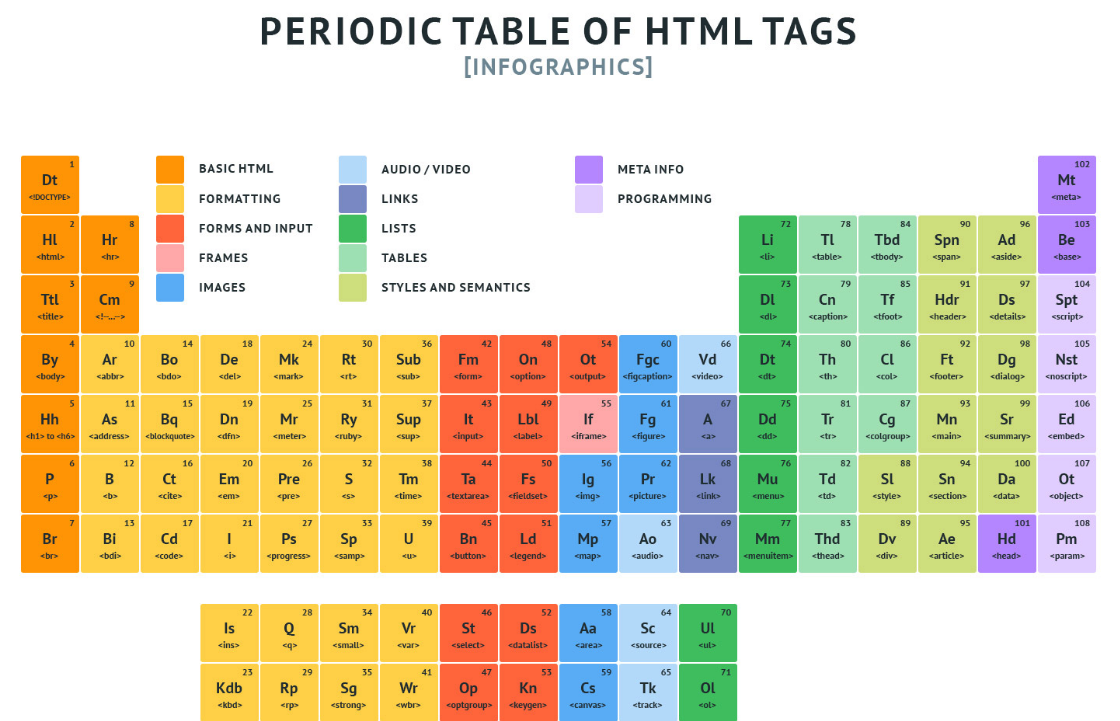
\includegraphics[width=\textwidth]{img/Screenshot_20200212_142612.png}
    \caption{Overzicht HTML tags}
\end{figure}



\subsubsection{Unclosed HTML tags}
\begin{itemize}
    \item Sommige HTML tags worden niet afgesloten
    \item Kunnen geen content bevatten
\end{itemize}
\begin{lstlisting}
<img src="yawningcat.gif" alt="Animated image of a yawning cat">
<input type="text">
\end{lstlisting}

\subsection {HTML attributes}
\begin{itemize}
    \item Definieert het gedrag van een tag
    \item Attributes moeten op de start tag
    \item Attributes kunnen 1 of meerdere values hebbben
    \item Globale attributes
    \item Specifieke attributes
\end{itemize}

\begin{lstlisting}
<elementattribute_name="value">content</element>
\end{lstlisting}

\subsubsection{HTML global attributes}
Kunnen op elke HTML tag geplaatst worden
\begin{itemize}
    \item class
    \item id
    \item \url{https://www.javatpoint.com/html-global-attributes}
\end{itemize}

\begin{lstlisting}
<h1id="value">content</h1>
<nav class="nav nav-main">content</nav>
\end{lstlisting}

\subsubsection{HTML specifieke attributes}
Kunnen op 1 specifieke HTML tag geplaatst worden 
\begin{itemize}
    \item href
    \item type
    \item src
\end{itemize}

\begin{lstlisting}
<a href="/index">content</a>
\end{lstlisting}

\subsubsection {Semantic tags}
\begin{itemize}
    \item Semantiek is de studie van de betekenis van woorden en bewoordingen in een taal. 
    \item Semantische elementen = elementen met betekenis.
    \item Een semantisch element beschrijft duidelijk de betekenis ervan voor zowel de browser als de ontwikkelaar.
    \item Voorbeelden van niet-semantische elementen: <div> en <span> - vertelt niets over de inhoud ervan.
    \item Voorbeelden van semantische elementen: <form>, <table> en <article>: definieert duidelijk de inhoud ervan.
\end{itemize}

\subsubsection {article}
\begin{itemize}
    \item Een zelfstandig onderdeel
    \item Is 'standalone' nog steeds zinvol
    \item Kan genest worden
    \item Kan meerdere sections, een header of footer bevatten
    \item Voorbeelden: 
    \begin{itemize}
        \item Forum post
        \item Blog post
        \item Newspaper article
    \end{itemize}
\end{itemize}

\subsubsection {section}
\begin{itemize}
    \item Beschrijft een sectie van een document
    \item Gerelateerde inhoud groeperen, als een onderdeel van een lang artikel, een groot deel van de pagina
    \item Heeft meestal een header en soms een footer
    \item Kan articles en sections bevatten
    \item Een homepage kan bijvoorbeeld opgesplitst worden in een intro section, een main content section en een contact section
\end{itemize}

\subsubsection {header}
\begin{itemize}
    \item Beschrijft een header van een document, section of article
    \item Container voor intro content
    \item Verschillende headers in 1 document
    \item Voorbeelden
    \begin{itemize}
        \item Header van een document met logo en navigatie
        \item Header van een article met intro content
    \end{itemize}
\end{itemize}

\subsubsection {footer}
\begin{itemize}
    \item Beschrijft een footer voor een document, section of article
    \item Extra informatie over het element waar de footer in zit
    \item Verschillende footer in 1 document
    \item Voorbeelden:
    \begin{itemize}
        \item Auteur, copyright informatie, extra links, contact informatie
        \item Deelknoppen van social media (bv binnen een article)
        \item Niet altijd onderaan!
    \end{itemize}
\end{itemize}

\subsubsection {nav}
\begin{itemize}
    \item Grote belangrijke navigatie links
    \item Primaire en secundaire informatie
    \item Enkel voor menu's
    \item Niet voor alle links
    \item Horizontaal of verticaal
    \item Bevat meestal een <ul> omdat het een lijst is van links
\end{itemize}

\subsubsection{aside}
\begin{itemize}
    \item Beschrijft content aside van een page/section content
    \item Binnenin section bvb poll, samenvatting
    \item Buiten article bvb commentatren, tweets, aside
\end{itemize}

\subsubsection{figure \& figcaption}
\begin{itemize}
    \item figcaption = voegt een visuele beschrijving toe aan een image
    \item <img> en <figcaption> zitten gegroepeerd in <figure>
\end{itemize}

\subsubsection{div}{
    \begin{itemize}
        \item W3C: \textit{generic container for flow content that by itself does not represent anything}
        \item Niet semantisch
        \item Enkel voor opmaak met css
    \end{itemize}
}

\subsubsection{span}{
    \begin{itemize}
        \item W3C: \textit{generic container for phrasing content that by itself does not represent anything}
        \item Niet semantisch
        \item Enkel voor opmaak met css
    \end{itemize}
}

\subsubsection{Block level element}
\begin{itemize}
    \item Start altijd op een nieuwe lijn 
    \item Neemt de volledige breedte in die mogelijk is
    \item Rekt zo ver mogelijk links en rechts uit 
    \item Is even breed als de breedte van het bovenliggende element/scherm/viewport
\end{itemize}

Voorbeelden:\\


\begin{figure}[H]
    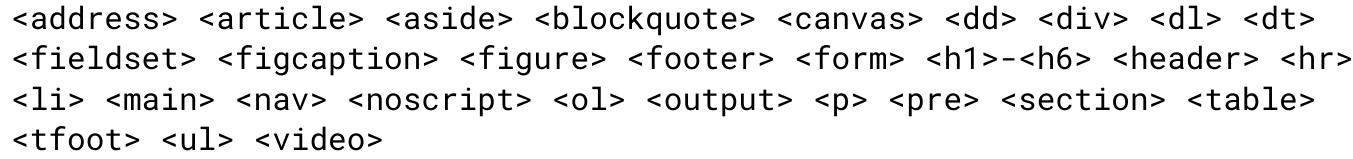
\includegraphics[width=0.9\textwidth]{img/Screenshot_20200212_144611.png}
\end{figure}




\subsubsection{Inline level element}
\begin{itemize}
    \item Start niet op een nieuwe lijn 
    \item Neemt enkel de breedte in die het nodig heeft
    \item Sommige CSS properties (width, height, padding, ...) doen niets.  
\end{itemize}

\subsection{The CSS Box Model}
\begin{itemize}
    \item Alle HTML elementen zijn boxes 
    \item Box-model bepaalt hoe de oppervlakte van een box worden berekend. 
    \item De oppervlakte: (van binnen naar buiten) 
    \item Content: de content van de box. Waar text en images komen.
    \item Padding: Ruimte rond de content. Is altijd transparant 
    \item Border: een border rond de padding en de content. Kan wel een kleur hebben 
    \item Margin: Extra ruimte buiten de border. Is altijd transparant
\end{itemize}

\subsubsection{Default rendering: box-model}
\begin{itemize}
    \item Width en height bepalen de grootte van de content
    \item Padding en border worden er niet bij opgeteld
    \item Margin duwt de box naar boven, rechts, beneden, of links waardoor de totaal ingenomen plaats ook beinvloed wordt
\end{itemize}

\subsubsection{Box-sizing: border-box}
\begin{itemize}
    \item Width en height bepalen de grootte van de content
    \item Padding en border worden vanbinnen toegevoegd en beïnvloeden dus niet langer de grootte van een element.
    \item Margin duwt de box naar boven, rechts, beneden of links waardoor de totale ingenomen plaats ook beïnvloedt wordt.
\end{itemize}

\subsection{Code conventions}
\begin{itemize}
    \item Geen ID's voor styling
    \item Lowercase tags
    \item Tags afsluiten
    \item Lowercase attribute names
    \item Attributen tussen dubbele aanhalingstekens
    \item Image attributes
    \item Indent
\end{itemize}

\section{CSS}
\begin{itemize}
    \item Cascading Style Sheet
    \item Taal om te specifieren hoe documenten (HTML) worden gerepresenteerd
    \item Browsers passen CSS rules uit de stylesheet toe op elementen van een document
    \item CSS rules bestaan uit:
    \begin{itemize}
        \item Selector
        \item Set van properties
    \end{itemize}
\end{itemize}

\subsection{Hoe werkt CSS?}
\begin{itemize}
    \item Een browser interpreteert een HTML document in 2 stadia:
    \begin{itemize}
        \item De browser converteert HTML en CSS in de Document Object Model (DOM). De DOM combineert de content met de stijl.
        \item De browser toont de content van de DOM
    \end{itemize}
\end{itemize}

\subsection{DOM (Document Object Model)}
\begin{itemize}
    \item De DOM representeert het document in het geheugen van de computer  
    \item DOM is where your CSS and the document's content meet up 
    \item Boom structuur 
    \item Elk element, attribuut en stukje tekst wordt een DOM node in de boom structuur 
    \item Nodes worden gedefinieerd door hun relatie tov andere DOM nodes 
    \item Parents \& Children
\end{itemize}




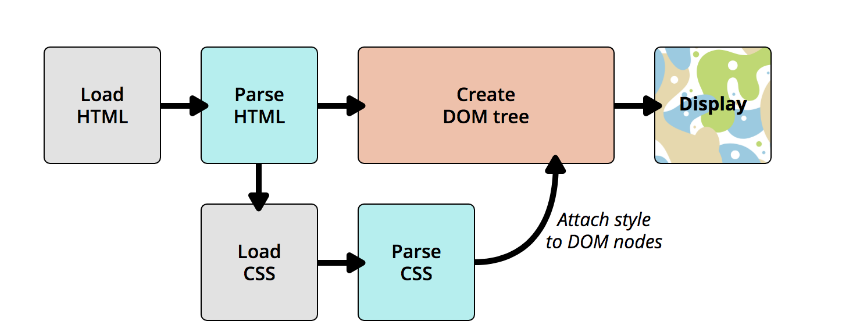
\includegraphics[width=0.9\textwidth]{img/Screenshot_20200212_151335.png}

\subsection{CSS Syntax}
\begin{itemize}
    \item CSS declaration 
    \begin{itemize}
        \item \bold{Properties:} Wat?
        \item \bold{Values:} Hoe?
    \end{itemize}
    \item CSS Declartion blocks
    \item CSS Ruleset/rule
\end{itemize}

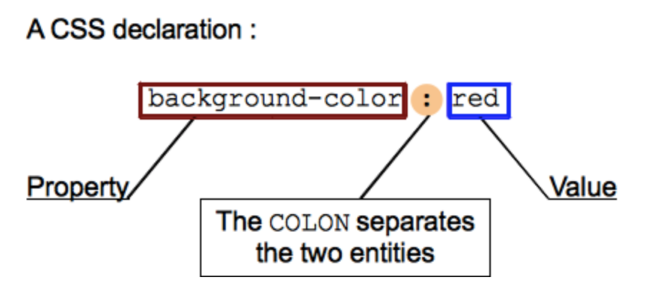
\includegraphics[width=0.9\textwidth]{img/Screenshot_20200212_151458.png}

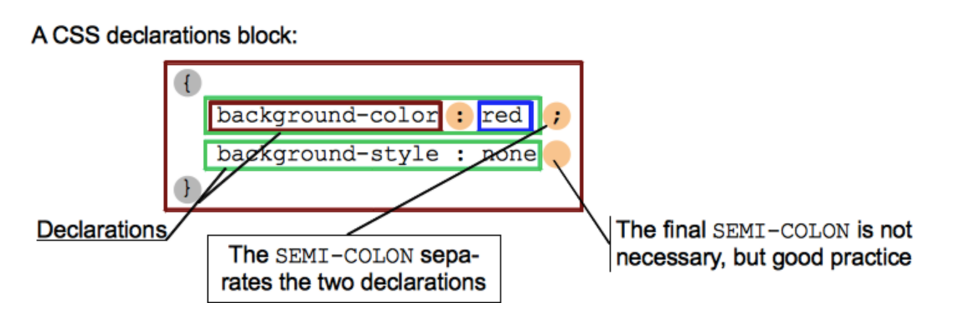
\includegraphics[width=0.9\textwidth]{img/Screenshot_20200212_151542.png}

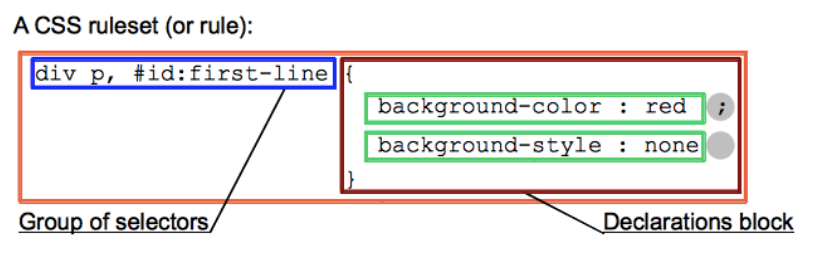
\includegraphics[width=0.9\textwidth]{img/Screenshot_20200212_151616.png}

\subsection{Selectors}
\begin{itemize}
    \item Simple selectors
    \begin{itemize}
        \item Type selectors (=element selectors): body, h1, p, ul, ...
        \item Class selectors: .class-name
        \item ID selectors: \#id-name
        \item Universal selector: *
    \end{itemize}
    \item Attribute selectors
    \begin{itemize}
        \item CSS rules worden toegepast op elementen met een bepaald attribuut en attribuut waarde. 
        \item Kan je herkennen aan de square brackets: [attr] 
        \item Presence and value attribute selectors 
        \item Substring value attribute selectors 
        \item Meer info: 
    \end{itemize}
    \url{https://developer.mozilla.org/en-US/docs/Learn/CSS/Introduction\_to\_CSS/Attribute\_selectors}

    \item Pseudo selectors
    \begin{itemize}
        \item pseudo-classes: selector\bold{:hover} 
        \item pseudo-elements: selector\bold{::before}
    \end{itemize}
    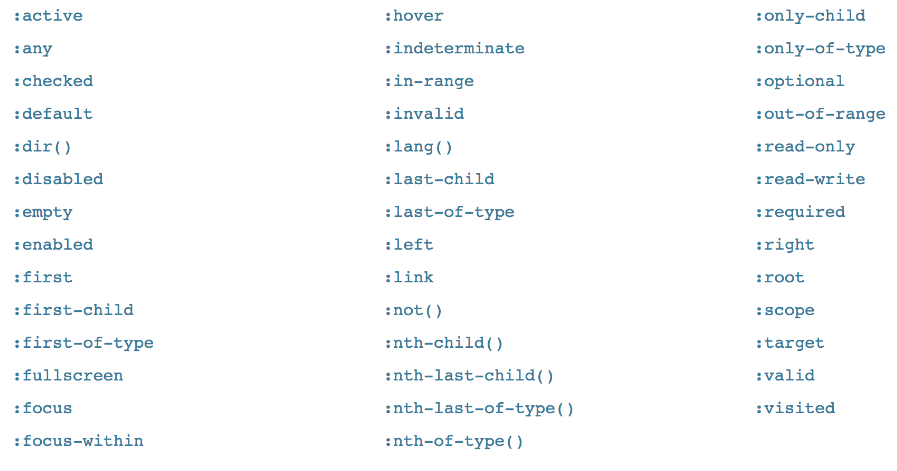
\includegraphics[width=0.9\textwidth]{img/Screenshot_20200212_152251.png}
    \item Combinators
    \begin{itemize}
        \item Group of selectors: A, B 
        \item Descendant selector: A B 
        \item Child selector: A $>$ B 
        \item Adjacent sibling selector: A + B 
        \item General sibling selector: A $\sim$ B
    \end{itemize}
    \item Multiple Selectors
\end{itemize}

\subsection{The Cascade}
\begin{itemize}
    \item Cascading: trapsgewijs
    \item Welke CSS rule wint? De volgorde:
    \begin{itemize}
        \item Source order
        \item Specificity
        \item Importance
    \end{itemize}
\end{itemize}

\subsubsection{Source Order}
\begin{itemize}
    \item Volgorde van CSS rules in de CSS file
    \item Van boven naar beneden
    \item Wat onderaan in de CSS staat wint van wat er boven staat
    \item Tenzij de specificity of importance hoger is.
\end{itemize}

\subsubsection{Specificity}
Hoe specifiek is een selector? De rangorde der selectors: 
\begin{enumerate}
    \item Element selectors
    \item Class selectors
    \item ID selectors
\end{enumerate}
Berekening van een waarde door middel van 4 scores:
\begin{itemize}
    \item \bold{1000: } inline styles
    \item \bold{0100: } voor elke id er in de selector voor komt
    \item \bold{0010: } voor elke class, attribute of pseudo class er in de selector voor komt
    \item \bold{0001: } voor elk element of pseudo element er in de selector voor komt
\end{itemize}

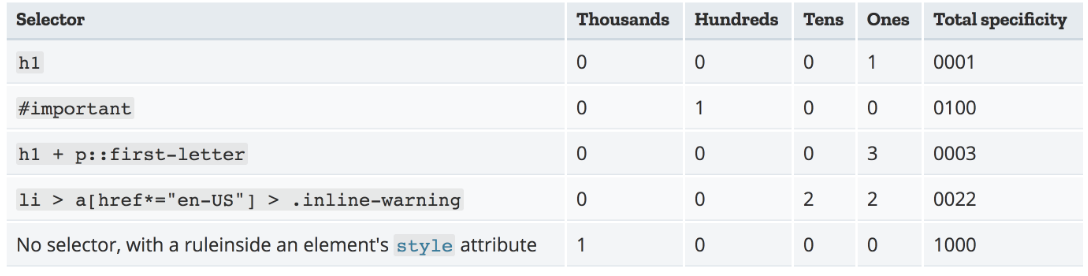
\includegraphics[width=0.9\textwidth]{img/Screenshot_20200212_152940.png}

\subsubsection{Importance}
Speciale syntax die al hetgeen hiervoor overschrijft: \textcolor{red}{!important}

\begin{lstlisting}
selector {     
    property: value !important; 
}
\end{lstlisting}

Zo weinig mogelijk gebruiken!

Hangt ook af van welke stylesheet de declaration in staat:
\begin{enumerate}
    \item Declarations in de user agent style sheets (browser default styles)
    \item Normale declarations in user style sheets (custom styles instellingen door een gebruiker). 
    \item Normale declarations in author style sheets (onze stylesheets). 
    \item Important declarations in author style sheets
    \item Important declarations in user style sheets
\end{enumerate}

\subsubsection{Rule mixin}
\begin{itemize}
    \item Properties overschrijven andere properties
    \item Niet de volledige CSS rule
\end{itemize}

\subsubsection{Inheritance}
\begin{itemize}
    \item Sommige property values die toegepast worden op een parent element worden overgenomen door de children van dat element.
    \begin{itemize}
        \item font-family
        \item color
        \item \dots
    \end{itemize}
    \item Sommige niet
    \begin{itemize}
        \item margin, padding, border, background image
    \end{itemize}
    \item Welke wel en welke niet is redelijk logisch
    \item Volledig overzicht: \url{https://developer.mozilla.org/en-US/docs/Web/CSS/Reference}
\end{itemize}

Je kan dat zelf forceren door:
\begin{lstlisting}
selector {     
    property: value; 
} 

selector child {
    property: inherit; 
}
\end{lstlisting}

\subsection{Code conventions}
\begin{itemize}
    \item Geen ID’s gebruiken om te stijlen 
    \item White space! 
    \item Laatste declaration ook een semi-colon geven; 
    \item Comments
    \item Shorthand properties
    \item Lowercase selectors
    \item Maximum 3 niveaus diep gaan met selectors
    \item Nog beter: zo veel mogelijk classesz
\end{itemize}

\underline{Zie Theorie 4.2 - CSS.pdf voor voorbeelden}

\section{CSS Defaults}

\subsection{User Agent Stylesheet}
\begin{itemize}
    \item Elke browser heeft een standaard stylesheet
    \item Om de pagina toch iets van stijl te geven 
    \item Verschilt van browser tot browser
    \item Tegenwoordig heel gelijkaardig
    \item Maar andere manier van interpretatie
\end{itemize}

\subsection{normalize.css}
\begin{itemize}
    \item Betere consistentie tussen browsers
    \item Creeert een standaardstijl voor HTML-elementen over alle browsers heen
    \item Alternatief voor reset.css
    \item Best practice
    \item Behoud nuttige browser-standaardinstellingen ipv ze te wissen
    \item Normaliseert stijlen voor een breed scala aan HTML-elementen
    \item Corrigeert bugs en algemene browser inconsistenties
    \item Verbetert de usability met subtiele verbeteringen
    \item Verklaart de code met behulp van comments en gedetailleerde documentatie
\end{itemize}

\subsection{reset.css}
\begin{itemize}
    \item Reset letterlijk alle elementen
    \item Alle elementen krijgen dezelfde kleur, dezelfde font-size, margin
    \item Opnieuw beginnen
\end{itemize}

\subsection{Vendor prefixes}
\begin{itemize}
    \item Vendor = browser maker
    \item Prefix = toevoeging aan de CSS-property
    \item CSS browser prefixes
    \item Support van CSS-features voor dat ze standaard worden. Bv: CSS-grid
    \item Geldt voornamelijk nog voor oudere browsers zoals IE10
    \item Prefixed properties eerst, normal properties laatst
    \item \url{shouldiprefix.com}
\end{itemize}

\bold{Prefixes:}

\begin{table}[H]
    \resizebox{0.3\textwidth}{!}{%
    \begin{tabular}{|l|l|}
    \hline
    \textbf{Browser}  & \textbf{prefix} \\ \hline
    Android           & -webkit-        \\ \hline
    Chrome            & -webkit-        \\ \hline
    iOS               & -webkit-        \\ \hline
    Safari            & -webkit-        \\ \hline
    Firefox           & -moz-           \\ \hline
    Internet Explorer & -ms-            \\ \hline
    Opera             & -o-             \\ \hline
    \end{tabular}%
    }
\end{table}

\subsection{caniuse.com}
\begin{itemize}
    \item Up-to-date browser support
    \item Front-end web technologieën
    \item Desktop en mobiele browsers 
    \item \url{https://caniuse.com/flexbox}
\end{itemize}


\subsection{Browser support}

\begin{itemize}
    \item Hangt af van project tot project
    \item Check Google Analytics om te zien met welke browser en OS bezoekers komen
    \item IE11 usage:
    \begin{itemize}
        \item Globaal: 1.55\%
        \item Belgie: 2\%
    \end{itemize}
\end{itemize}

\subsubsection{Desktop Browsers}
Laatste versie van \underline{evergreen browsers} - browsers die zichzelf updaten:
\begin{itemize}
    \item Chrome
    \item Safari
    \item Firefox
    \item Opera
\end{itemize}

Laatste versie van Microsoft Edge en Internet Explorer

\subsubsection{Mobiele Browsers}
Standaar browser van de laatste versie van OS.
\begin{itemize}
    \item iOS 13: \bold{Safari}
    \item Android 9 \& 10: \bold{Chrome}
    \item IE mobile 11
\end{itemize}

\subsection{Progressive enhancement}
\begin{itemize}
    \item Manier om te ontwikkelen
    \item Basis level van UX die nodig is voor je applicatie
    \item Meer geavanceerde functionaliteit als de browser het ondersteunt
    \item CSS fallbacks
    \begin{itemize}
        \item = CSS die gebruikt wordt als geavanceerde functionaliteit niet wordt ondersteund door de browser
    \end{itemize}
\end{itemize}

\subsection{Margin collapsing}
\begin{itemize}
    \item Standaard krijgt elk typografisch element een margin-top en bottom
    \item \bold{Maar} die worden niet opgeteld
    \begin{itemize}
        \item Margins van opeenvolgende elementen worden niet opgeteld
        \item Margins van elementen in een parent met ook een parent worden niet opgeteld
        \item Grootste margin = totale verticale margin
    \end{itemize}
\end{itemize}
= collapsing margins


\subsection{Margin \& Padding baseline system}
\bold{Verticale white space tussen block level tekst elementen:}
\begin{itemize}
    \item single-direction margin declarations
    \item Alle margins duwen in dezelfde richting
    \item margin-bottom
    \item Veelvoud van de baseline
\end{itemize}

\subsection{Het verschil tussen margin en padding?}
\begin{itemize}
    \item \bold{Padding} voegt witruimte toe binnen de box
    \item \bold{Margin} voegt witruimte toe buiten de box
\end{itemize}

\subsubsection{Margin \& padding system gebaseerd op de baseline}
\begin{itemize}
    \item Vertical white space tussen grote blokken: padding-top en bottom
    \item padding-top = padding-bottom x 2
    \item Horizontal white-space tussen columns en rand van de viewport of container: padding-left en -right
    \item Padding-left en -right: meervoud van de baseline
\end{itemize}

\subsection{Units of measurement: EM vs REM vs PX}
\begin{itemize}
    \item pixels: absoluut. Een pixel is een pixel. Kan niet groter of kleiner worden
    \item Relatief:
    \begin{itemize}
        \item em: 1em = 1x de font-size van de parent
        \item rem = root em = 1x de font-size van de root (het html element)
        \item Worden uiteindelijk ook berekend als pixels door de browser
    \end{itemize}
\end{itemize}

\subsubsection{Voorbeelden}
\begin{lstlisting}
.voorbeeld{
    font-size: 3rem;
    max-width: 20em;
}

\end{lstlisting}


\begin{lstlisting}
html {
    font-size: 100%; /* 16px */
}
    
.klasse {
    font-size: 2em; /* 16*2 = 32px */
}

.klasse p {
    font-size: 2em; /* 32*2 = 64px */
}

\end{lstlisting}

\underline{Zie voorbeelden Theorie 5.1 - CSS defaults}


\section{CSS Architecture}
\subsection{CSS architecture}
\begin{itemize}
    \item Hoe schrijven we CSS?
    \item Schaalbaar en uitbereidbaar
    \item Onderhoudbaar
    \item De cascade onder controle houden
    \item Specificity Wars vermijden
\end{itemize}

\subsection{Specificity wars}
\begin{itemize}
    \item Welke selector wint hangt af van:
    \begin{itemize}
        \item De locatie in de css file
        \item De specificiteit van een selector
        \item Important
    \end{itemize}
    \item Locatie en specificiteit door elkaar gebruiken zorgt voor specificity wars
    \item Issues wanneer zwaardere selectors voor lichtere komen
\end{itemize}

\begin{figure}[H]
    \centering
    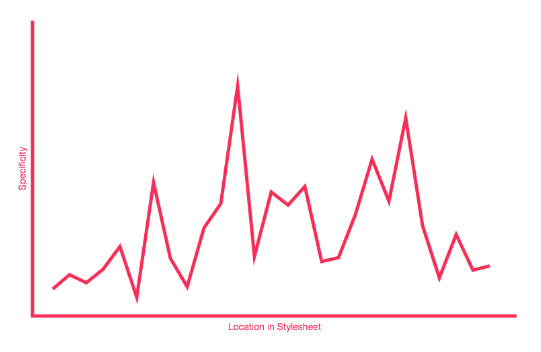
\includegraphics[width=0.3\textwidth]{img/Screenshot_20200309_101014.png}
    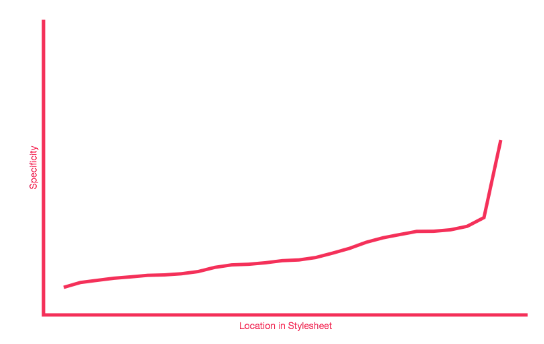
\includegraphics[width=0.3\textwidth]{img/Screenshot_20200309_101053.png}
    \caption{Specificity graphs: rechts is beter}
\end{figure}


\subsection{ITCSS}
\begin{itemize}
    \item = Inverted Triangle CSS
    \item Manier om CSS te schrijven
    \item In volgorde van specificiteit
    \begin{itemize}
        \item Eerst element selectors rulesets
        \item Daarna class selectors rulesets
    \end{itemize}
    \item Bouwt verder op elkaar en voegt enkel toe of erft over van wat er voor komt
    \item Harry Roberts: CSS Wizardry
    \item \url{https://www.cssguidelin.es}
\end{itemize}

\begin{figure}[H]
    \centering
    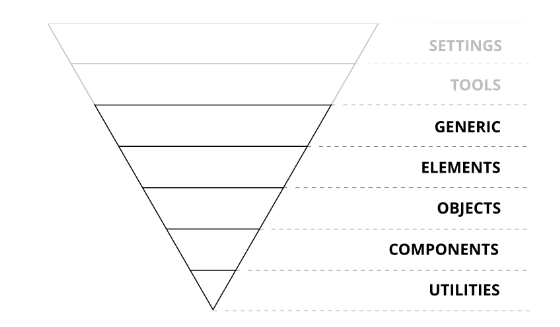
\includegraphics[width=0.3\textwidth]{img/Screenshot_20200309_101408.png}
    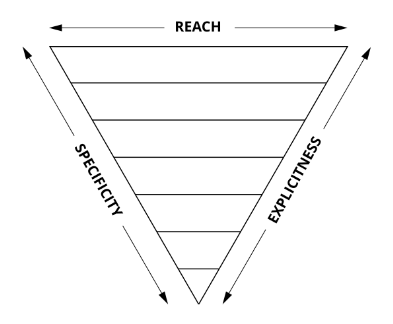
\includegraphics[width=0.3\textwidth]{img/Screenshot_20200309_101427.png}
    \caption{Inverted traingle}
\end{figure}

\begin{itemize}
    \item \bold{Generic:} reset/normalize.css, universal selector * voor box sizing
    \item \bold{Elements:} styling voor pure HTML elementen zoals H1, A, etc...
    \item \bold{Objects:} herbruikbare class selectors die basis stijlen voor bepaalde patronen definieren (zoals een grid systeem)
    \item \bold{Components:} herkenbare specifieke UI components met class selectors 
    \item \bold{Utilities:} Class selectors met 1 specifiek doel die alles kunnen overschrijven die in de voorgaande layers zit. Kan zelfs !important bevatten
\end{itemize}

\subsection{Class naming conventions}
\begin{itemize}
    \item Moeilijkste deel van css schrijven: naamgeving
    \item Altijd lowercase
    \item Woorden scheiden door koppelteken
    \item Namespacing system
    \item Baseren op ITCSS structuur
\end{itemize}

Types

\begin{itemize}
    \item Object classes: .o-
    \item Component classes: .c-
    \item Scoping classes: .s-
    \item Utility classes: .u-
    \item Javascript hooks: .js-
\end{itemize}

\subsubsection{Object classes .o-}
\begin{itemize}
    \item Herbruikbare class selectors die basis stijlen voor bepaalde patronen definieren (zoals een grid systeem)
    \item Kunnen voorgedefinieerd zijn in je css boilerplate, herbruikbaar voor ieder project
    \item .o-layout, .o-list
\end{itemize}

\subsubsection{Component classes .c-}
\begin{itemize}
    \item Herkenbare specifieke UI components
    \item Zijn specifiek per project
    \item .c-nav
    \item .c-button
    \item .c-author
\end{itemize}

\subsubsection{Scoping classes .s-}
\begin{itemize}
    \item Het is niet altijd mogelijk om aan elk element een class te geven
    \item CMS component
    \item Elementen scopen binnen een bepaalde context
    \item .s-content
\end{itemize}

\subsubsection{Utility classes .u-}
\begin{itemize}
    \item Class selectors met 1 specifiek doel en die alles kunnen overschrijven die in de voorgaande layers zit
    \item Kunnen voorgedefinieerd zijn in je css boilerplate, herbruikbaar voor ieder project
    \item .u-text-center
    \item .u-max-width-large
\end{itemize}

\subsubsection{Javascript hooks .js-}
\begin{itemize}
    \item Manier om duidelijk te maken in de HTML dat aan dit element javascript gekoppeld is. Verwijderen heeft dus geen impact
    \item Styling en functionaliteit scheiden
    \item .js-toggle-mobile-nav
    \item .js-show-next
\end{itemize}

\subsection{BEM-notatie: Block element, modifier}
Manier van naamgeving om object en component classes te groeperen en modulair te maken
\begin{itemize}
    \item \bold{Block:} Op zichzelf staande entiteit die op zich betekenisvol is. De parent node
    \item \bold{Element:} Een deel van een block dat geen zelfstandige betekenis heeft en dat semantisch is verbonden met het block. De child node.
    \item \bold{Modifier:} Voegt kleine veranderingen toe op blocks of elements bovenop hun bestaande properties
    \item \bold{+ITCSS class namespacing}
\end{itemize}

In CSS:
\begin{itemize}
    \item .block
    \item .block\_\_element
    \item .block--modifier
    \item .block\_\_element--modifier
\end{itemize}

\begin{lstlisting}
.c-body{
    ...
}

.c-body__arm {
    ...
}

.c-body__arm--left {
    ...
}

.c-body__arm--right {
    ...
}
\end{lstlisting}

Real life examples:
\begin{itemize}
    \item Navigatie
    \item Buttons
    \item Grid system
    \item \dots
\end{itemize}

\subsubsection{Rules}
\begin{itemize}
    \item Maximum 1 element diep
    \item Als een element kan opgedeeld worden in andere elementen: maak een nieuwe block aan
    \item Niet nesten met css als het niet nodig is
    \item Modifiers kunnen niet op zich staan
\end{itemize}

\subsection{Goede CSS selector}
\begin{itemize}
    \item Is niet te specifiek
    \item Is overdraagbaar naar andere elementen
    \item Is herbruikbaar
    \item Is locatie onafhankelijk
    \item Is duidelijk maar toch vaag
    \item Niet nesten als het niet nodig is
\end{itemize}

\subsubsection{Selector intent}
\begin{itemize}
    \item Wat is het doel van je selector
    \item Selecting the right things for the right reasons
    \item Wat wil je stijlen en hoe ga je dat doen?
    \item \bold{Bijvoorbeeld:} stijlen van de primaire navigatie van een website
\end{itemize}

\subsubsection{Overdraagbaarheid}

\begin{itemize}
    \item Geen \bold{Qualified selectors} gebruiken
    \item Overdraagbaar naar andere elementen
\end{itemize}

\subsubsection{Locatie onafhankelijk}

\begin{itemize}
    \item Geen stijlen toepassen op elementen op basis van waar ze zich bevinden
    \item Maar op basis van wat ze zijn
    \item Zo worden ze locatie onafhankelijk
\end{itemize}


\subsubsection{Naming}

\begin{itemize}
    \item Kies namen die gemakkelijk te onderhouden zijn
    \item In plaats van heel specifieke namen
    \item Die duidelijk zijn maar toch vaag
\end{itemize}

\subsection{The Single Responsibility Principle}

\begin{itemize}
    \item Development in het algemeen
    \item Elk stukje code focust zich op 1 iets
    \item Kleine CSS classes die zich focussen op 1 iets specifiek
    \item UI's opdelen tot in de kleinste component die 1 verantwoordelijkheid heeft
    \item Combinatie van die componenten tot grote complexe constructies
\end{itemize}

\subsection{The seperation of concerns}

\begin{itemize}
    \item Lijkt heel goed op \textit{the single responsibility principle}
    \item HTML \& CSS opdelen in duidelijk te onderscheiden section
    \item Individuele componenten die 1 taak verzorgen
    \item Samenstellen van al die verschillende componenten vormt de volledige UI
    \item Bijvoorbeeld een grid system voor layout
\end{itemize}

\subsection{CSS selectors in MCT}
\begin{itemize}
    \item Elements en classes
    \item Opdelen in objecten en componenten, utilities om heel specifieke zaken te overschrijven
    \item Namespacing prefixes: .o-, .c-, .u- voor class selectors
    \item BEM notatie voor class selectors
    \item Makkelijk te onderhouden en uitbereidbaar
    \item Specificity wars voorkomen
\end{itemize}

\section{Flexbox}
\subsection{Zelfstudie}
\begin{itemize}
    \item Interactieve tutorial: \url{https://scrimba.com/g/gflexbox}
    \item Demo 1: \url{https://codepen.io/simoncoudeville-nmct/pen/zYGpJjz}
    \item Demo 2: \url{https://codepen.io/simoncoudeville-nmct/pen/bGdLJGj}
\end{itemize}

\subsection{CSS Flexible Box Layout Module}
\begin{itemize}
    \item Creëert een Flexible box zoals een Inline box of een Block box.
    \item display: flex;
    \item Methode voor het positioneren van elementen in horizontale of verticale stacks.
    \item Efficiënte manier om elementen naast elkaar te plaatsen, te spreiden en te aligneren
    \item Voor kleine, 1 dimensionale layouts.
    \item CSS Grid voor grotere, 2 dimensionale layouts.
    \item Met de flex layout model kunnen directe children van een flex container in gelijk welke richting gelayout worden.
    \item Flex container: parent - eigen properties
    \item Flex items: direct children - eigen properties
    \item flex-flow directions
    \item Main-axis
    \item Cross-axis
\end{itemize}

\begin{figure}[H]
    \centering
    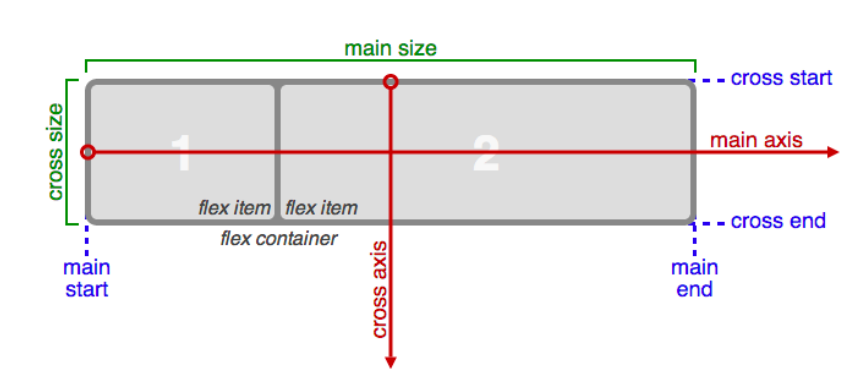
\includegraphics[width=0.7\textwidth]{img/Screenshot_20200330_112142.png}
    \caption{Flex container}
\end{figure}

\subsection{Properties voor de parent (flex container)}

\begin{itemize}
    \item \bold{display:} flex | inline-flex
    \item \bold{flex-direction:} row | row-reverse | column | column-reverse;
    \item \bold{flex-wrap:} nowrap | wrap | wrap-reverse;
    \item \bold{flex-flow:} $<$'flex-direction'$>$ || $<$'flex-wrap'$>$;
    \item \bold{justify-content:} flex-start | flex-end | center | space-between | space-around | space-evenly;
    \item \bold{align-items:} flex-start | flex-end | center | baseline | stretch;
    \item \bold{align-content:} flex-start | flex-end | center | space-between | space-around | stretch;
\end{itemize}

\subsection{Display}
Creëert een block of inline element voor de container en een flex layout voor de children.

\begin{lstlisting}
display: flex            =     display: block flex;
display: inline-flex     =     display: inline flex;
\end{lstlisting}

\subsection{Flex-direction}
\begin{itemize}
    \item Bepaalt de direction van de main-axis
    \item Bepaalt de positie van de main-start
    \item Bepaalt waar de flow van de items start.
    \item Bepaalt zo de volgorde van de elementen.
    \item \bold{Values:}
    \begin{itemize}
        \item row
        \item row-reverse
        \item column
        \item column-reverse
    \end{itemize}
\end{itemize}

\begin{figure}[H]
    \centering
    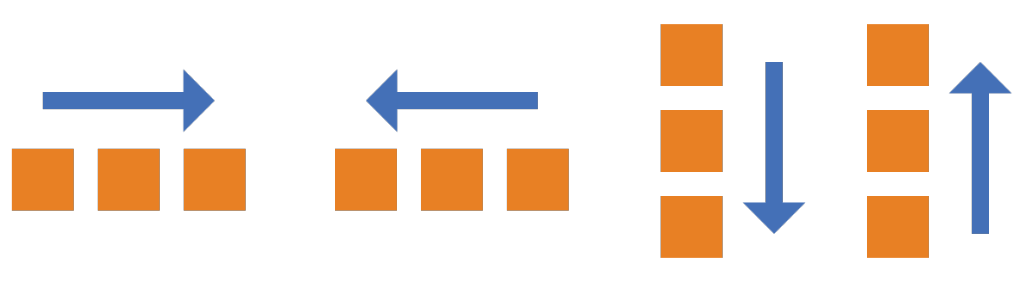
\includegraphics[width=0.7\textwidth]{img/Screenshot_20200330_112728.png}
    \caption{Flex direction}
\end{figure}

\begin{figure}[H]
    \centering
    
\includegraphics[width=0.6\textwidth]{img/Screenshot_20200427_092621.png}
    \caption{Flex direction: row}
\end{figure}

\begin{figure}[H]
    \centering
    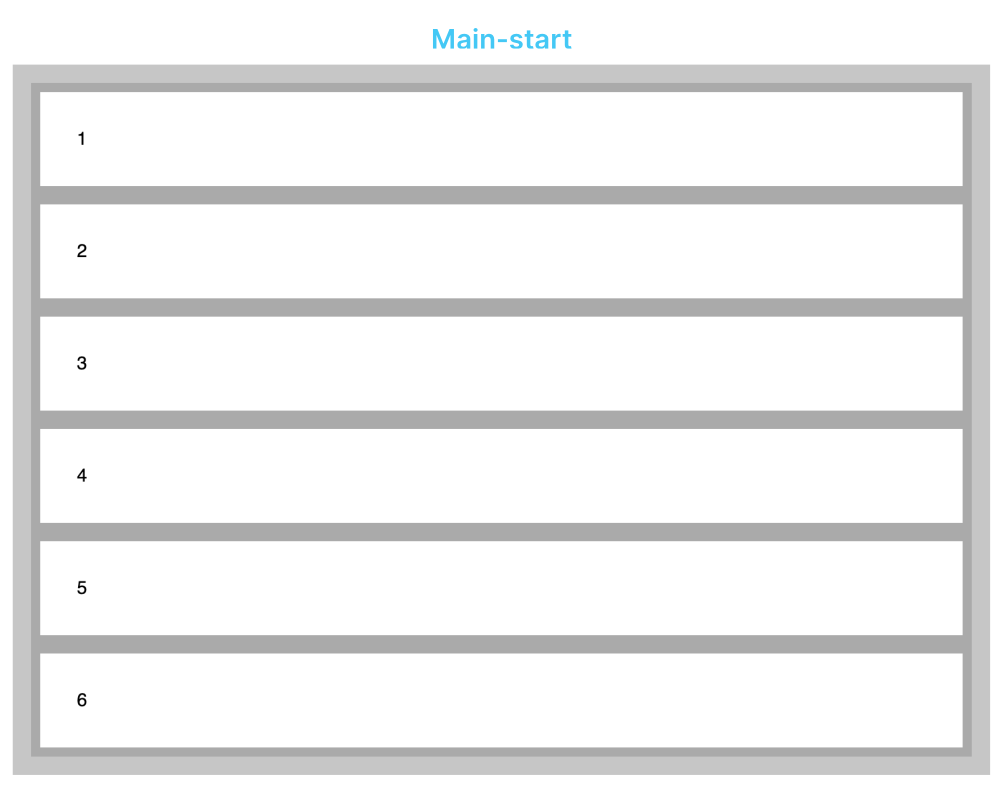
\includegraphics[width=0.4\textwidth]{img/Screenshot_20200427_092708.png}
    \caption{Flex direction: column}
\end{figure}

\begin{figure}[H]
    \centering
    
\includegraphics[width=0.6\textwidth]{img/Screenshot_20200427_092800.png}
    \caption{Flex direction: row-reverse}
\end{figure}


\subsubsection{flex-direction: column-reverse}
= identiek aan row-reverse, maar met een column

\subsection{Flex-wrap}
\begin{itemize}
    \item Bepaalt of een flex-container single-line of multi-line is.
    \item Bepaalt richting van de cross-axis, in welke richting nieuwe lines lopen.
\end{itemize}

\begin{figure}[H]
    \centering
    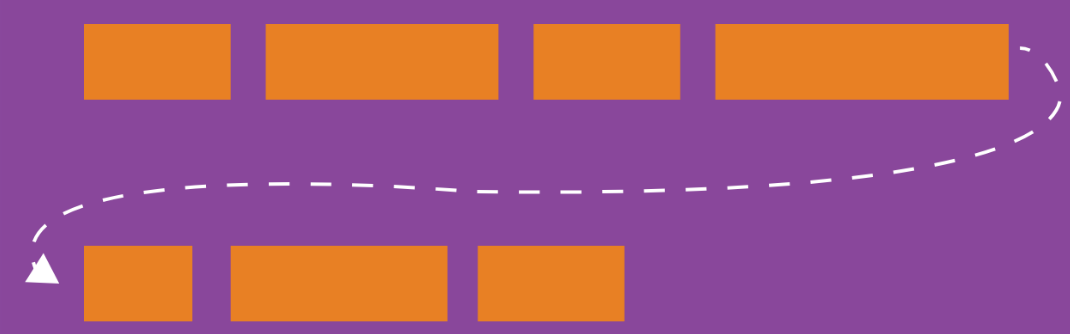
\includegraphics[width=0.4\textwidth]{img/Screenshot_20200427_092927.png}
    \caption{Flex-wrap}
\end{figure}

Values:

\begin{itemize}
    \item no-wrap: Items worden altijd naast elkaar gezet. (default)
    \item wrap: items komen onder elkaar indien nodig
    \item wrap-reverse: items komen onder elkaar en de cross axis wordt omgedraaid.
\end{itemize}

\begin{figure}[H]
    \centering
    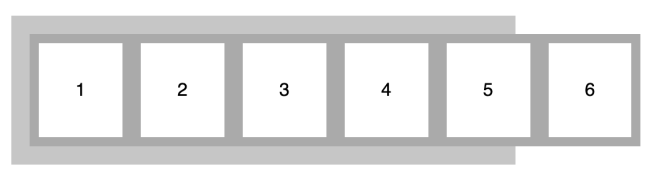
\includegraphics[width=0.3\textwidth]{img/Screenshot_20200427_093040.png}
    \caption{Flex-wrap: no-wrap (default)}
\end{figure}

\begin{figure}[H]
    \centering
    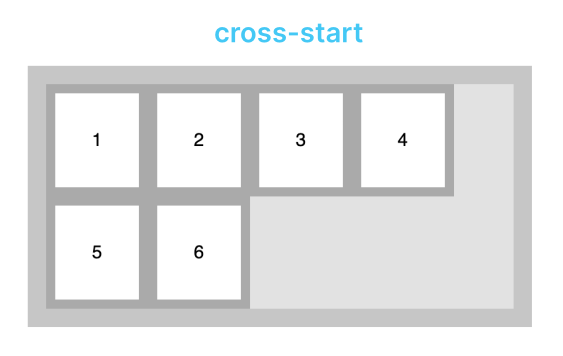
\includegraphics[width=0.3\textwidth]{img/Screenshot_20200427_093104.png}
    \caption{Flex-wrap: wrap}
\end{figure}

\begin{figure}[H]
    \centering
    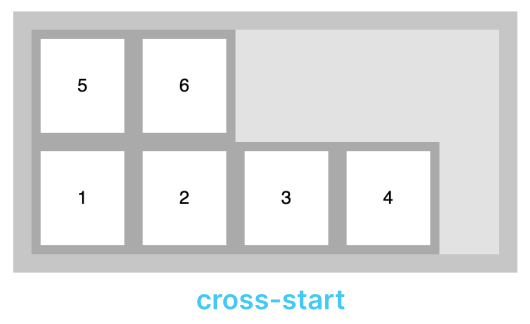
\includegraphics[width=0.3\textwidth]{img/Screenshot_20200427_093216.png}
    \caption{Flex-wrap: wrap-reverse}
\end{figure}

\subsection{Justify-content}

Bepaalt de alignment van de items op de main-axis.
Heeft alleen effect als de breedte van de container breder is dan alle items.

\bold{Values:}
\begin{itemize}
    \item flex-start: main-start (default)
    \item flex-end: main-end
    \item center: in het midden van de main-axis
    \item space-around, space-between, space-evenly
\end{itemize}


\begin{figure}[H]
    \centering
    
\includegraphics[width=0.4\textwidth]{img/Screenshot_20200427_093349.png}
    \caption{Justify-content: flex-start}
\end{figure}

\begin{figure}[H]
    \centering
    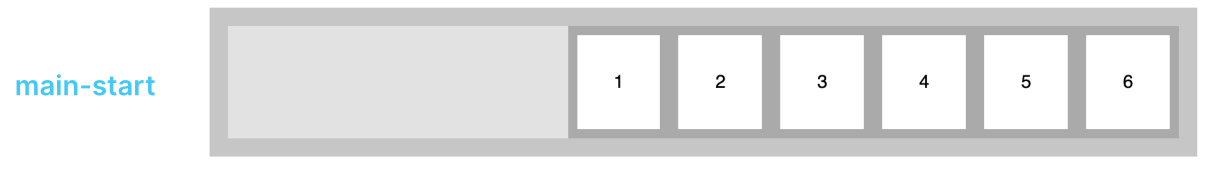
\includegraphics[width=0.4\textwidth]{img/Screenshot_20200427_093608.png}
    \caption{Justify-content: flex-end}
\end{figure}

\begin{figure}[H]
    \centering
    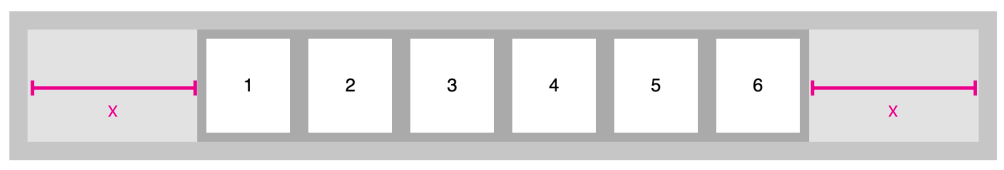
\includegraphics[width=0.4\textwidth]{img/Screenshot_20200427_093729.png}
    \caption{Justify-content: center}
\end{figure}

\begin{figure}[H]
    \centering
    
\includegraphics[width=0.4\textwidth]{img/Screenshot_20200427_093753.png}
    \caption{Justify-content: space-between}
\end{figure}

\begin{figure}[H]
    \centering
    
\includegraphics[width=0.4\textwidth]{img/Screenshot_20200427_093824.png}
    \caption{Justify-content: space-around}
\end{figure}

\begin{figure}[H]
    \centering
    
\includegraphics[width=0.4\textwidth]{img/Screenshot_20200427_093901.png}
    \caption{Justify-content: space-evenly}
\end{figure}


\subsection{Align-items}
Bepaalt de alignment van de items op de cross-axis

\bold{Values:}
\begin{itemize}
    \item stretch: maakt items even hoog (default)
    \item flex-start: cross-start
    \item flex-end: cross-end
    \item center: in het midden van de cross-axis
    \item baseline
\end{itemize}

\begin{figure}[H]
    \centering
    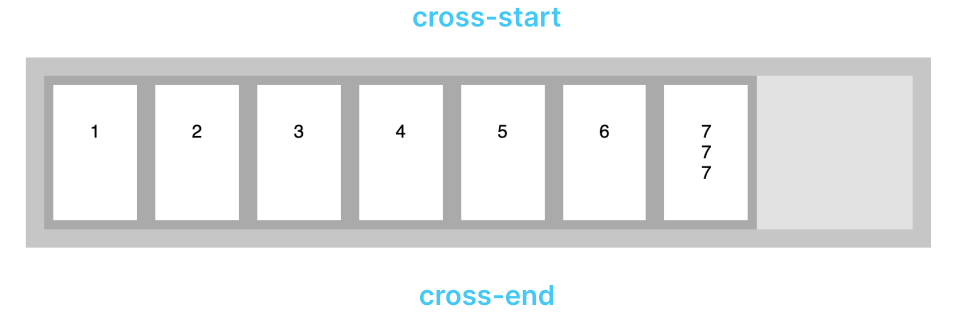
\includegraphics[width=0.4\textwidth]{img/Screenshot_20200427_094108.png}
    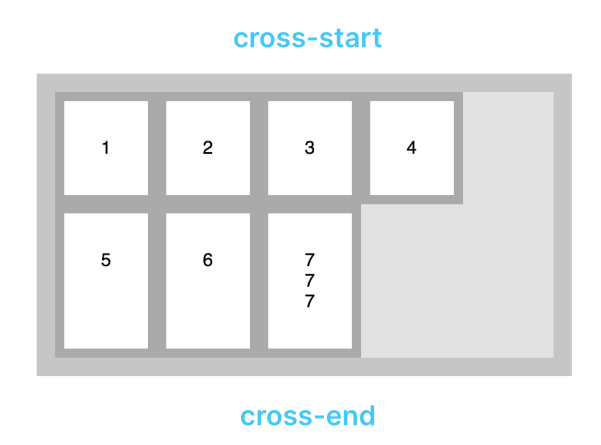
\includegraphics[width=0.4\textwidth]{img/Screenshot_20200427_094153.png}
    \caption{align-items: stretch (default)}
\end{figure}

\begin{figure}[H]
    \centering
    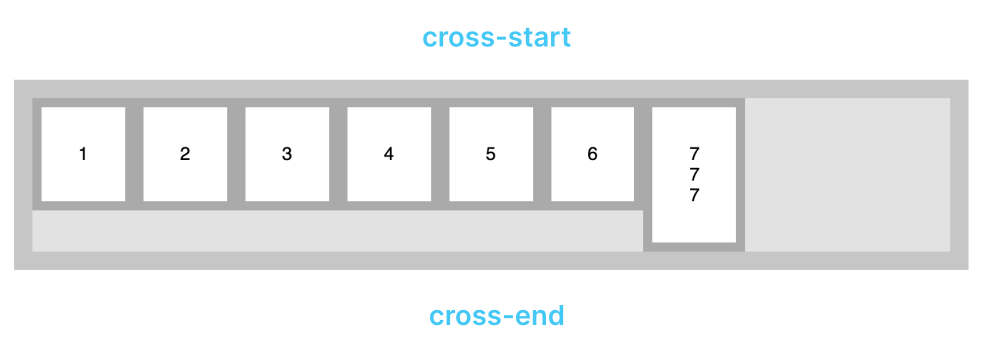
\includegraphics[width=0.4\textwidth]{img/Screenshot_20200427_094237.png}
    \caption{align-items: flex-start}
\end{figure}

\begin{figure}[H]
    \centering
    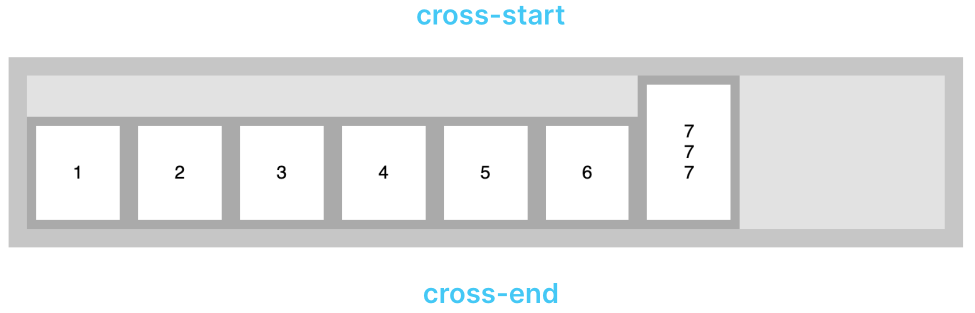
\includegraphics[width=0.4\textwidth]{img/Screenshot_20200427_094305.png}
    \caption{align-items: flex-end}
\end{figure}

\begin{figure}[H]
    \centering
    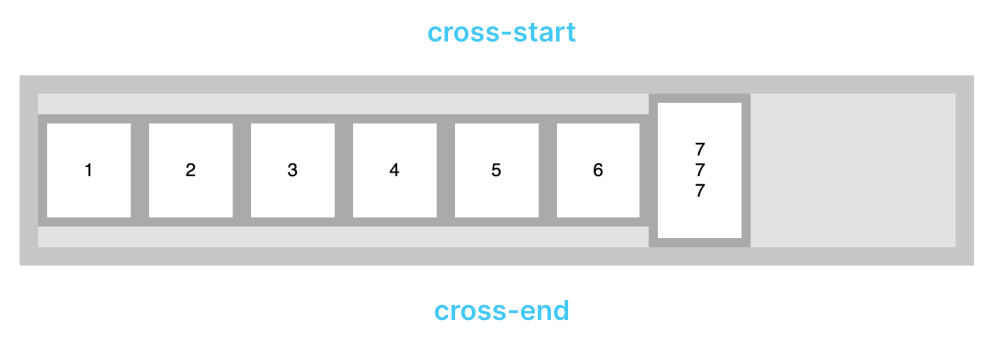
\includegraphics[width=0.4\textwidth]{img/Screenshot_20200427_094327.png}
    \caption{align-items: center}
\end{figure}

\begin{figure}[H]
    \centering
    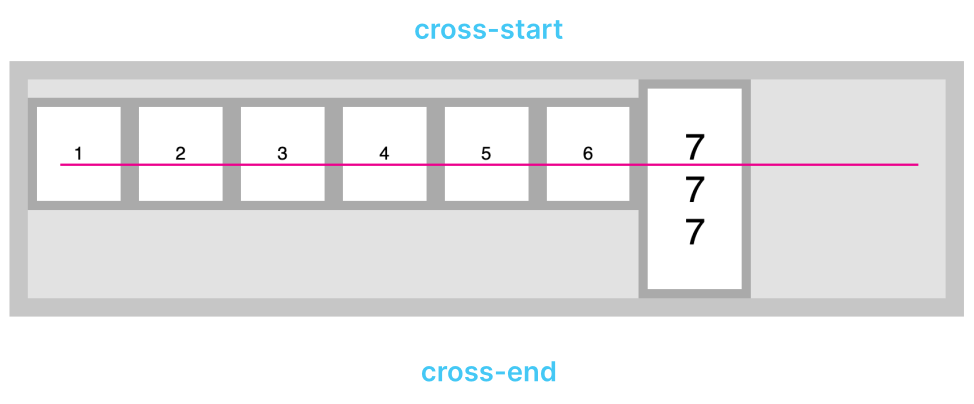
\includegraphics[width=0.4\textwidth]{img/Screenshot_20200427_094349.png}
    \caption{align-items: baseline}
\end{figure}


\subsection{Align-content}

Bepaalt de container van de items op de cross-axis met meerdere lijnen tov de container.

\begin{itemize}
    \item Werkt enkel als de container hoger is dan alle items samen
    \item Er moeten meerdere lijnen zijn
\end{itemize}

\bold{Values}
\begin{itemize}
    \item stretch: items op dezelfde lijn worden even hoog (default)
    \item flex-start: cross start
    \item flex-end: cross end
    \item center: in het midden van de cross-axis
    \item space-around, space-between \& space-evenly
\end{itemize}

\subsection{Properties voor de flex items}
\begin{lstlisting}
order: <integer>;
align-self: auto | flex-start | flex-end | center | baseline |
stretch;
flex-grow: <number>; /* default 0 */
flex-shrink: <number>; /* default 1 */
flex-basis: <length> | auto; /* default auto */
flex: none | [ <'flex-grow'> <'flex-shrink'> || <'flex-basis'> ] /*
default 0 1 auto*/
\end{lstlisting}

\subsubsection{Order}
\begin{itemize}
    \item Bepaalt de visuele order van 1 item.
    \item Als alle andere items standaard op order: 0 staan wordt het item helemaal naar achter verplaatst.
\end{itemize}

\begin{lstlisting}
.c-layout__item:nth-child(1) {
    order: 1;
    border-color: red;
    color: red;
}
\end{lstlisting}

\begin{figure}[H]
    \centering
    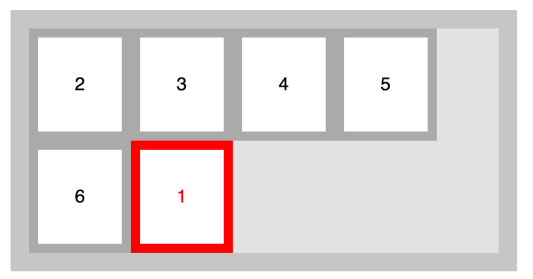
\includegraphics[width=0.4\textwidth]{img/Screenshot_20200427_095803.png}
    \caption{Voorbeeld Order}
\end{figure}

\subsection{Align-self}
Hierdoor kan de alignment die is gespecificeerd door align-items worden overschreven voor individuele flex items.

\bold{Values:}
\begin{itemize}
    \item auto /* default: volgt align-items */
    \item flex-start
    \item flex-end
    \item center
    \item baseline
    \item stretch
\end{itemize}

Deze values werken exact zoals align-items en align-content, maar dan op individuele flex items.

Bv: align-self: center:

\begin{lstlisting}
.c-layout__item:nth-child(5) {
    align-self: center;
}
\end{lstlisting}

\begin{figure}[H]
    \centering
    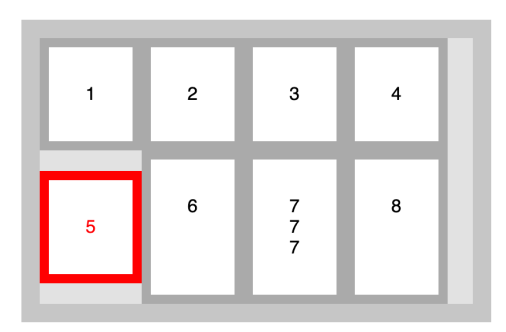
\includegraphics[width=0.4\textwidth]{img/Screenshot_20200427_100049.png}
    \caption{Voorbeeld align-self}
\end{figure}

\subsection{flex}
Hoe items flexen is afhankelijk van:
\begin{itemize}
    \item Aantal items
    \item Breedte van de container
    \item \bold{Content van de items}
\end{itemize}

\begin{figure}[H]
    \centering
    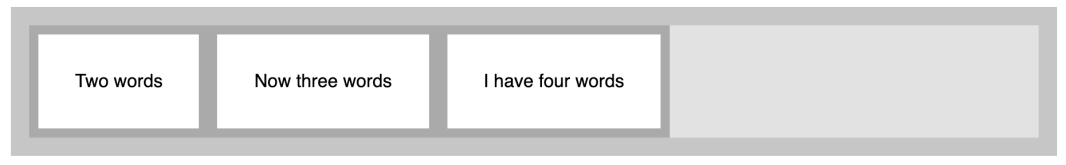
\includegraphics[width=0.45\textwidth]{img/Screenshot_20200427_101021.png}
    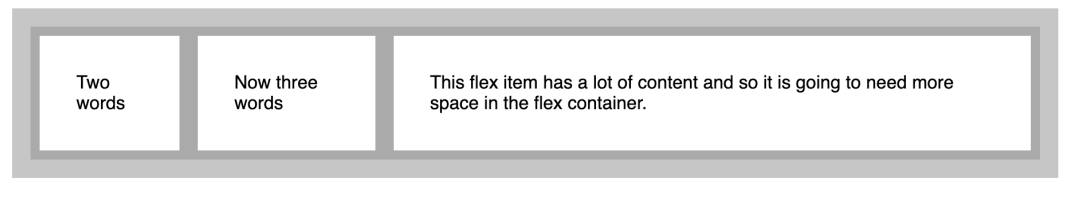
\includegraphics[width=0.45\textwidth]{img/Screenshot_20200427_100955.png}
    \caption{Flex is afhankelijk van de content van de items}
\end{figure}

\begin{lstlisting}
flex: 0 1 auto
\end{lstlisting}
Standaard voor alle flex-items

Shorthand voor:
\begin{lstlisting}
flex-grow: 0
flex-shrink: 1
flex-basis: auto
\end{lstlisting}

\subsubsection{Flex-grow}
\begin{lstlisting}
flex-grow: 0
\end{lstlisting}

\begin{itemize}
    \item Items worden standaard niet groter om de beschikbare plaats in te nemen op de main-axis.
    \item Negatieve nummers kunnen niet
\end{itemize}

\begin{figure}[H]
    \centering
    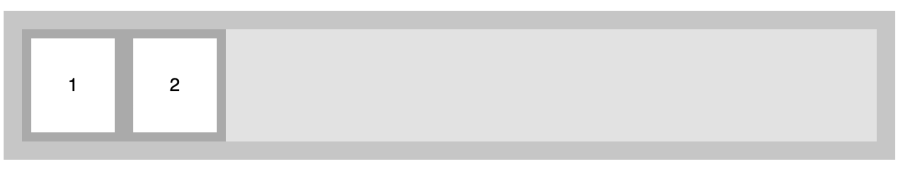
\includegraphics[width=0.45\textwidth]{img/Screenshot_20200427_101411.png}
    
\includegraphics[width=0.45\textwidth]{img/Screenshot_20200427_101400.png}
    \caption{flex-grow: 0 vs flex-grow: 1}
\end{figure}


\begin{figure}[H]
    \centering
    
\includegraphics[width=0.6\textwidth]{img/Screenshot_20200502_195208.png}
    
\end{figure}
\begin{figure}[H]
    \centering
    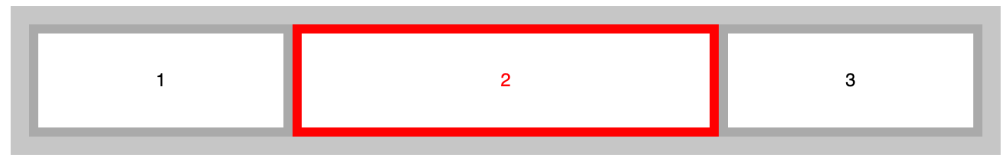
\includegraphics[width=0.6\textwidth]{img/Screenshot_20200502_195358.png}
\end{figure}
\begin{figure}[H]
    \centering
    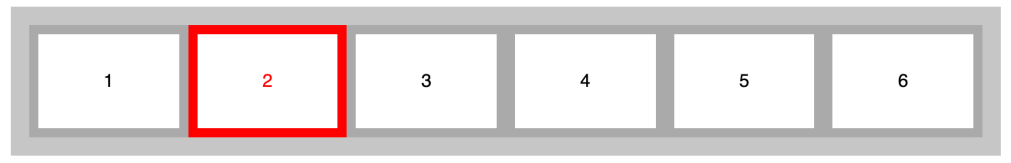
\includegraphics[width=0.6\textwidth]{img/Screenshot_20200502_195446.png}
    \caption{Alle elementen hebben een flex-grow van 1, het 2de element heeft een flex-grow van 2}
\end{figure}

\subsubsection{Flex-shrink}

\begin{itemize}
    \item flex-shrink: 0;
    \begin{itemize}
        \item Items worden niet kleiner, er ontstaat overflow
    \end{itemize}
    \item flex-shrink: 1;
    \begin{itemize}
        \item Items zullen zo klein mogelijk worden voor er overflow gebeurt.
        \item Negatieve nummers kunnen niet.
    \end{itemize}
\end{itemize}

\subsubsection{Flex-basis}

Bepaalt de default size van een element voor de overgebleven ruimte wordt verdeeld.

\begin{itemize}
    \item flex-basis: auto; (default)
    \begin{itemize}
        \item Zorgt voor de best mogelijke layout.
        \item Groot genoeg om de content te laten passen.
        \item Hangt af van de flex-grow property.
        \item Hangt ook af of items wrappen of niet.
    \end{itemize}
    \item flex-basis: 0;
    \begin{itemize}
        \item items worden maar zo groot als het langste woord van de content.
    \end{itemize}
    \item flex-basis: 200px;
    \begin{itemize}
        \item een item zal nooit kleiner worden dan 200px, eventueel wel groter
    \end{itemize}
    \item flex-basis: 50\%: 
    \begin{itemize}
        \item een item zal nooit kleiner worden dan 50\% van de container, eventueel wel groter
    \end{itemize}
    \item Geen negatieve waarden mogelijk
\end{itemize}

\subsubsection{Resources}

\begin{itemize}
    \item \url{https://css-tricks.com/snippets/css/a-guide-to-flexbox/}
    \item \url{https://scrimba.com/g/gflexbox}
    \item \url{https://philipwalton.github.io/solved-by-flexbox/}
\end{itemize}


\section{Kleurtheorie}
\subsection{Hoe worden kleuren opgebouwd?}

\bold{Additief}
\begin{itemize}
    \item Licht
    \item RGB
    \item Alle kleuren samen zijn wit
    \item Digitaal
\end{itemize}

\bold{Subtractief}
\begin{itemize}
    \item Verf
    \item CMYK
    \item Alle kleuren samen zijn zwart
    \item Drukwerk
\end{itemize}

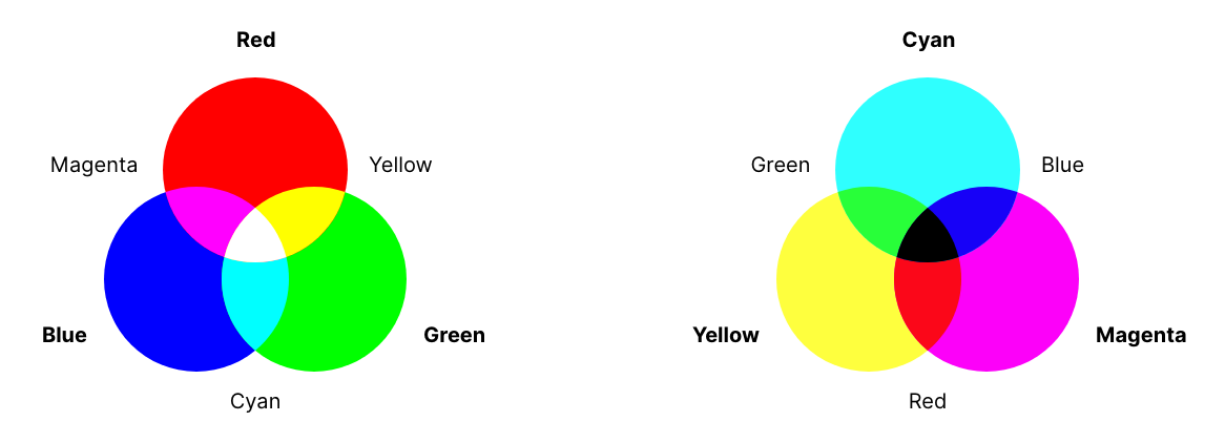
\includegraphics[width=0.9\textwidth]{img/Screenshot_20200217_083625.png}

\subsection{Additive color synthesis}
\begin{itemize}
    \item Gelijke verhouding van 2 primaire kleuren worden gecombineerd om de secundaire kleuren te creeren.
    \item Gelijke verhouding van 3 primaire kleuren worden gecombineerd om achromatische kleuren (wit, grijstinten en zwart) te creeren. 
\end{itemize}
Alle tinten van het zichtbare lichtspectrum zijn mengsels van verschillende verhoudingen van 1, 2, of 3 van de primaire lichtkleuren.
Een RGB-monitor synthetiseert kleuren additief door de rode, groene en blauwe 'phosphor-dots' van elke pixel selectief te verlichten met verschillende intensiteitsniveaus.

Het licht van de 3 phosphor-dots van een pixel smelt samen om 1 enkele kleur te genereren.


\subsubsection{Soorten kleuren}
\begin{itemize}
    \item \bold{Primary colors} : RGB
    \item \bold{Secundary colors} : Bestaat uit gelijke proporties van 2 primaire kleuren
    \item \bold{Achromatic colors} : Bestaat uit gelijke proporties van alle 3 de primaire kleuren
    \item \bold{Intermediate colors} : Bestaat uit gelijke proporties van opeenvolgende primaire en secundaire kleuren
\end{itemize}

\subsection{Hexadecimale codes}
Elke primaire kleur (RGB) heeft een bereik tussen 0 - 255. 
Voor de berekening van de hexadecimale waarde deel je de numerieke waarde van een kleur door 16 (=eerste deel).
De rest van de deling vormt het tweede deel van de hexadecimale waarde. 
Als de quötient of de rest van de deling groter is dan 9, dan wordt deze aangeduid met een letter A tot F (A: 10, B:11, C:12, D:13, E:14, F: 15)


\subsection{Color Properties}
\bold{Chromatic colors} : alle kleuren behalve wit, grijstinten en zwart - hebben 3 dimensies of eigenschappen:
\begin{enumerate}
    \item \bold{Hue} : 
    \begin{itemize}
        \item Een waarneembare kleur die overeenkomt met een unieke, dominante golflengte van licht
        \item De kleur van een object zoals waargenomen door het oog, ontstaan doordat één of twee primaire RGB-kleuren overheersen.
    \end{itemize}
    \item \bold{Value/Brightness} :
    \begin{itemize}
        \item De relatieve lichtheid of donkerheid van een kleur
    \end{itemize}
    \item \bold{Chroma/Saturation} : 
    \begin{itemize}
        \item De relatieve zuiverheid en intensiteit van een chromatic color. 
        \item Minder saturation is het wegnemen van kleur.
    \end{itemize}
\end{enumerate}

\subsubsection{HSB: Hue, Saturation Brightness}
\begin{itemize}
    \item Maakt het iets natuurlijker om een kleur te 'maken'
    \item \bold{Bv}: voor lichtere, donkere en minder gesatureerde kleuren.
\end{itemize}

\subsection{Kleurenpalet samenstellen}
\begin{itemize}
    \item Op gevoel
    \item Kleur samples
    \item Gebruik kleurenregels
    \item Tools
\end{itemize}

\subsubsection{Kleurenpalet}
\begin{itemize}
    \item \bold{Monochromatic of eenkleurig}: 1 kleur kiezen en saturation en brightness aanpassen om meerdere kleuren te maken
    \item \bold{Analogus of analoog}: naast elkaar liggende kleuren kiezen
    \item \bold{Complementary of complementair}: tegenovergestelde kleuren die elkaar aanvullen gebruiken
    \item \bold{Split complementary}

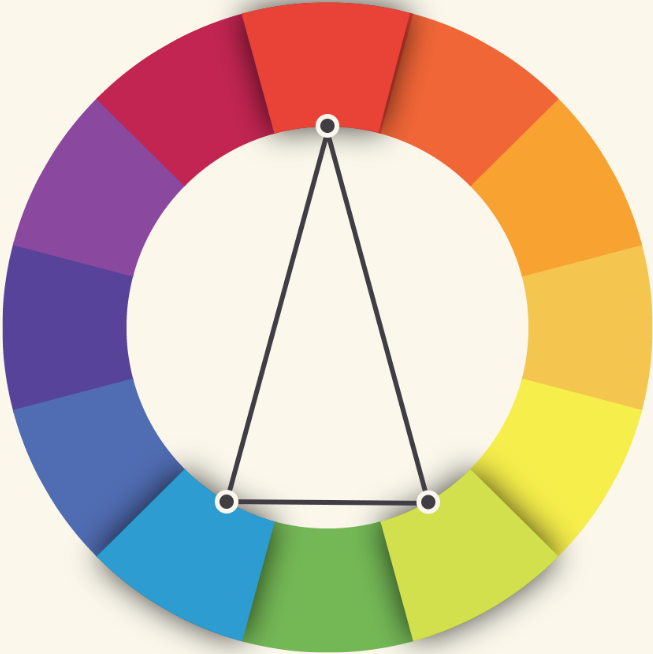
\includegraphics[width=0.2\textwidth]{img/Screenshot_20200217_092108.png}
    \item \bold{Triadic}
    
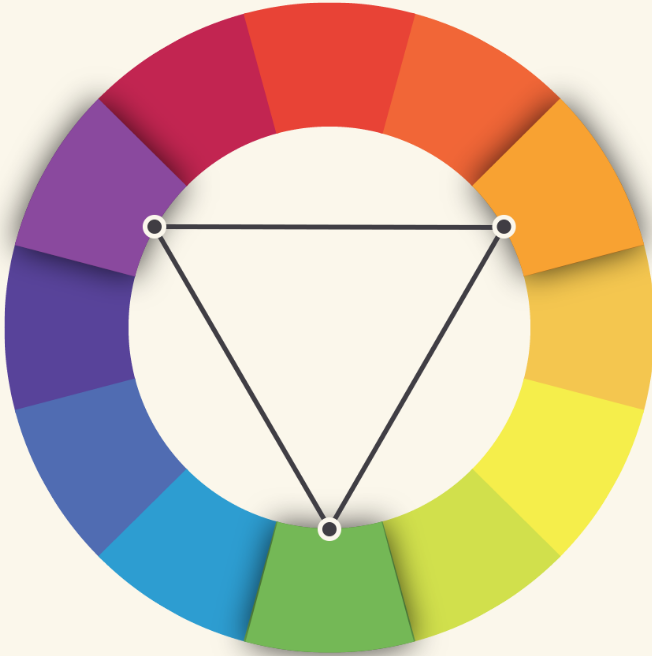
\includegraphics[width=0.2\textwidth]{img/Screenshot_20200217_092125.png}
    \item \bold{Tetradic}
    
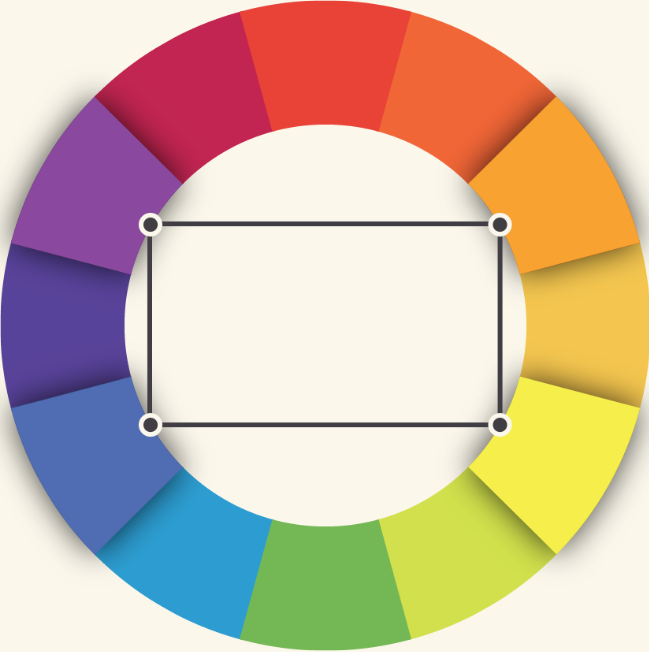
\includegraphics[width=0.2\textwidth]{img/Screenshot_20200217_092143.png}
\end{itemize}



\subsection{Kleurenpsychologie}

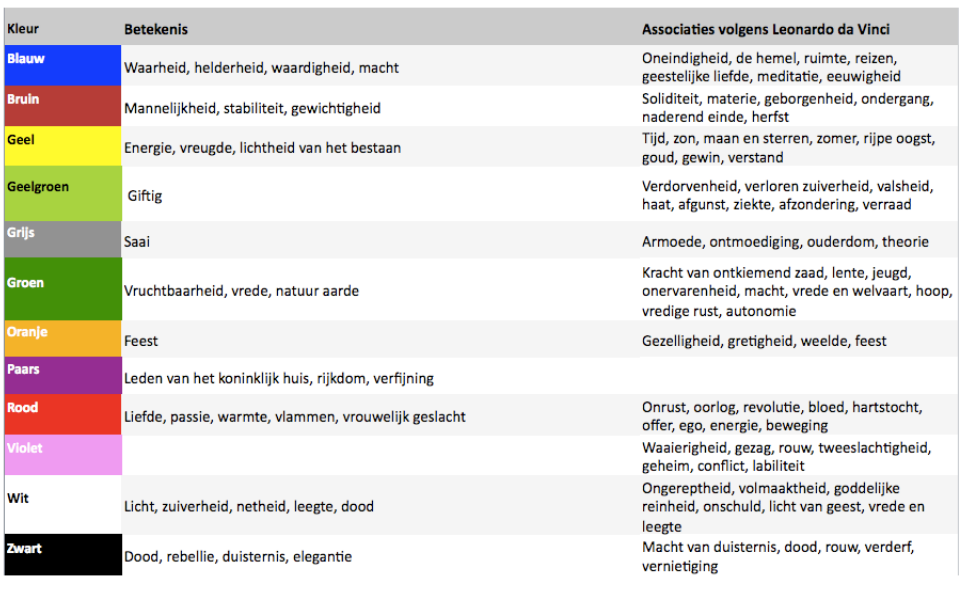
\includegraphics[width=\textwidth]{img/Screenshot_20200217_092401.png}

\begin{itemize}
    \item Rood: Bloed, liefde, oorlog
    \item Oranje: Speels, vrolijk voor kinderen
    \item Geel: vriendelijkheid, geluk, attentie, waarschuwingsborden
    \item Groen: groei, natuur, geld
    \item Blauw: betrouwbaar
    \item Paars: luxe
    \item Roze: vrolijkheid, jeugd, onschuld
\end{itemize}

\subsection{Contrast}
Zorg dat er een groot genoeg verschil tussen \bold{saturation} en \bold{brightness} is.

\subsubsection{Contrast ratio}
\begin{itemize}
    \item Volg accessibility standards outlined in de WCAG, de Web Content Accessibility Guidelines van W3C.
    \item Contrast ratio voor kleine tekst en grote tekst
    \item \bold{Kleine tekst}: kleiner dan 24px of 19px bold
    \item \bold{Grote tekst}: groter dan 24px of groter dan 19px bold
    \item 2 levels: AA and the more strict AAA
    \item Geen perfecte berekening: soms fouten
\end{itemize}

\bold{AA}
\begin{itemize}
    \item kleine tekst: minstens 4.5
    \item grote tekst: minstens 3 
\end{itemize}

\bold{AAA}
\begin{itemize}
    \item Strikter dan AA
    \item kleine tekst: minstens 7
    \item grote tekst: minstens 4.5
\end{itemize}

\subsubsection{Non-text contrast}
Componenten moeten een contrast ratio van minimaal 3: 1 hebben t.o.v. hun achterliggende achtergrond. 

\subsubsection{Interface elements}
Tekst t.o.v. achtergrond: minstens contrast ratio van 3:1
Background t.o.v. achterliggend element: minstens contrast ratio van 3:1
Als het kan: 
\begin{itemize}
    \item Kleine tekst bold zetten
    \item Background kleur donkerder zetten
    \item Font size vergroten
\end{itemize}

\subsubsection{Tekst}
\begin{itemize}
    \item minstens 4.5:1
    \item Grote tekst 3:1
\end{itemize}

\subsection{Kleurenblindheid}
\begin{itemize}
    \item "Druk op groen om door te gaan" = fout
    \item Zorg ervoor dat kleuren niet de enige manier zijn om belangrijke informatie over te brengen.
\end{itemize}
    

\subsection{Kleur in UI design}
\begin{itemize}
    \item Donkerdere kleur variaties worden gemaakt door de helderheid te verlagen en de verzadiging te verhogen
    \item Lichtere kleur variaties worden gemaakt door de helderheid te verhogen en de verzadiging te verlagen.
    \item We behouden zo veel mogelijk HUE.
\end{itemize}

\subsubsection{Tools}
\begin{itemize}
    \item \url{http://color.adobe.com/nl/create/color-wheel}
    \item \url{http://coolors.co/}
\end{itemize}

\section{Layout \& Grids}

\subsection{Layout}
\begin{itemize}
    \item De manier waarop een pagina wordt ingedeeld
    \item Hoe componenten op een pagina worden gepositioneerd
    \begin{itemize}
        \item Logo
        \item Navigatie
        \item Verschillende titels en tekst
        \item \dots
    \end{itemize}
\end{itemize}

\subsection{Alignment}
Ervoor zorgen dat elk element correct is gepositioneerd t.o.v. andere elementen.

\subsection{Grids}
\begin{itemize}
    \item Vormen de basis van een layout
    \item Zorgen voor orde en consistentie
    \item Versnellen het design proces
    \item Horizontal grid
    
    \item Vertical grid
    
\end{itemize}

\subsubsection{Horizontal Grid}
\begin{itemize}
    \item Van links naar rechts
    \item Columns
    \begin{itemize}
        \item Percentueel
        \item Afhankelijk van de breedte van de container
    \end{itemize}
    \item Breedtes
    \item Horitontale whitespace
    \item Verdeeld layout in grote stukken
    \item Container
    \begin{itemize}
        \item Smartphone scherm of browser of de maximum breedte die je instelt
    \end{itemize}
    \item Gutters (= whitespace tussen 2 items)
    \begin{itemize}
        \item Vaste waarde (24px, 30px, \dots) afhankelijk van spacing systeem
    \end{itemize}
\end{itemize}

\subsubsection{Vertical Grid}
\begin{itemize}
    \item Van boven naar onder
    \item Rows
\end{itemize}

\subsection{Grid systems}
\begin{itemize}
    \item 12-column grid
    \begin{itemize}
        \item Deelbaar door 2,3 en 4
        \item Minder kolommen beschikbaar
    \end{itemize}
    \item 16-column grid
    \begin{itemize}
        \item Deelbaar door 2 en 4
    \end{itemize}
    \item Niet te veel op vastpinnen: afwijken mag, met CSS kan alles
    \item 8/16 of 6/12 = 50\%
    \item 3/12 of 4/16 = 1/4 = 25\%
    \item 4/12 = 1/3 = 33.33\%
    \item Dus als je in een pagina 3 kolommen nodig hebt dan kan dat, ongeacht het grid system.
\end{itemize}


\subsubsection{Responsive grid}
\begin{itemize}
    \item Default van links naar rechts
    \item Wat er rechts niet meer bij kan verschuift bij een bepaald breakpoint naar onder
\end{itemize}

\subsubsection{Baseline grid}
\begin{itemize}
    \item Vertical grid
    \item Van boven naar onder
    \item Rows
    \item Hoogte
    \item Vertical white space boven en onder componenten
    \item Vertical rhythm
    \item 1 virtuele lijn die zich herhaald om de X aantal pixels
    \item Vermenigvuldigen om \dots:
    \begin{itemize}
        \item \dots hoogtes te bepalen
        \item \dots vertical white space boven en onder elementen te bepalen
    \end{itemize}
    \item In plaats van lukraak iets te plaatsen
\end{itemize}

\subsection{Spacing system}

\begin{itemize}
    \item 1 basis unit waarmee je kan vermenigvuldigen
    \item Basis voor horizontale white space zoals grid gutters
    \item Basis voor de verticale white space boven en onder componenten
    \item \bold{Voorbeeld}:
    \begin{itemize}
        \item Basis unit = 8px
        \item Column gutter = 3 * 8px = 24px
        \item Vertical margin = 3 * 8px = 24px
        \item 8px - 16px - 24px - 32px - \dots
    \end{itemize}
    \item Eens dit vast staat, overal in het design gebruiken voor alles wat met groottes en afstand te maken heeft
\end{itemize}

\subsection{White space}
\begin{itemize}
    \item De lege plaats tussen de items
    \item Padding
    \item Margin
    \item \url{https://scrimba.com/p/prpYaAy/c9BGgbC4}
\end{itemize}

\section{Typografie}
\begin{itemize}
    \item Typography transforms language into a decorative visual element.
    \item Web design is 95\% typografie
\end{itemize}

\subsection{Lettertype vs Font}
Lettertype = volledige design met alle varianten (zoals een album)
Font = 1 variant ervan (zoals een nummer op een album)

\subsection{Classificatie}
\begin{itemize}
    \item Serif
    \item Sans-serif
    \item Monospaced
    \item Decorative
    \item \url{https://betterwebtype.com/assets/pdf/better-web-type-font-styles-cheat-sheet.pdf}
\end{itemize}

\subsubsection{Serif}


\includegraphics[width=0.6\textwidth]{img/Screenshot_20200224_084536.png}

\begin{itemize}
    \item Schreef
    \item Zijn karakters met afsluitende streepjes (schreven) aan het eind van de letterbalken
    \item Vormen een denkbeeldige horizontale lijn, dat de leesbaarheid verbeterd
    \item Traditioneel
    \item Drukwerk: boeken, kranten
    \item Digitaal gebruiken voor titels en body copy
    \begin{itemize}
        \item Blogposts
        \item Nieuwsartikel
    \end{itemize}
    \item Niet voor kleine UI elementen
\end{itemize}


\bold{Types:}
\begin{itemize}
    \item Old style
    \item Transitional
    \item Neoclassical \& Didone
    \item Slab
    \item Clarendon
    \item Glypic
\end{itemize}

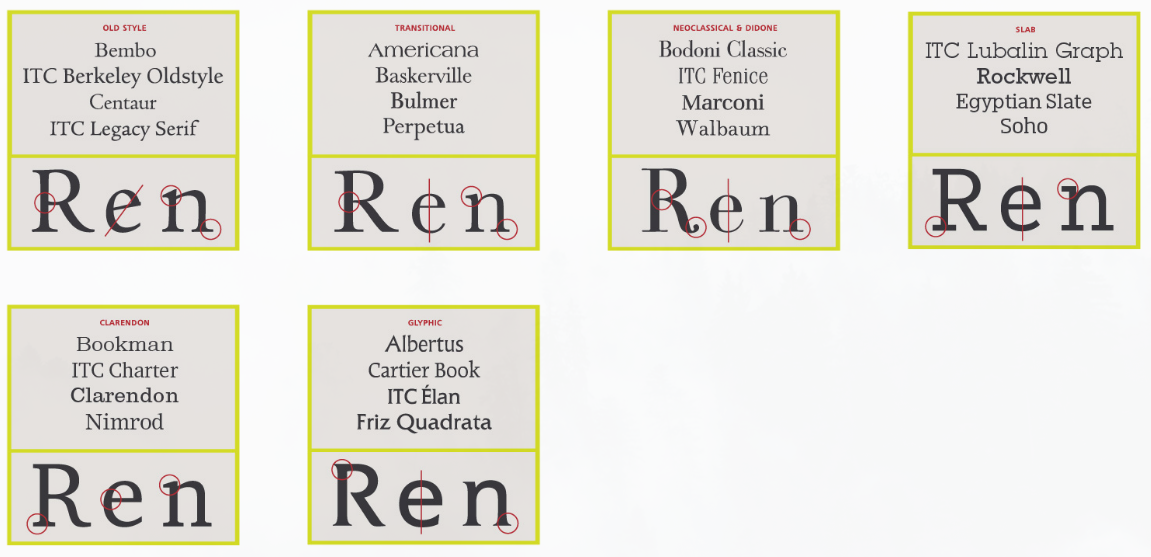
\includegraphics[width=0.9\textwidth]{img/Screenshot_20200224_084930.png}

\subsubsection{Sans-serif}
\begin{itemize}
    \item Schreefloze letter
    \item Letters zonder afsluitende streepjes aan het eind van de letterbalken
    \item Nieuwer innovatiever
    \item Perfect voor alles van tekst
    \item Perfect voor kleine UI elementen
\end{itemize}

\bold{Types:}
\begin{itemize}
    \item Grotesque \& Neo Grotesque
    \item Square
    \item Humanistic
    \item Geometric
\end{itemize}

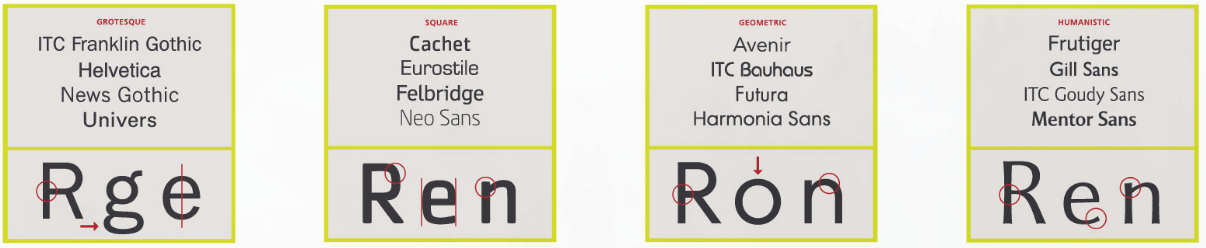
\includegraphics[width=0.9\textwidth]{img/Screenshot_20200224_085146.png}

\subsection{Monospaced}
\begin{itemize}
    \item Alle karakters nemen even veel plaats in
    \item Neemt dus meer plaats in 
    \item Veel gebruikt om code te schrijven
    \item Estetisch aantrekkelijk of niet? Kan over gediscussieerd worden
    \item Voor development: text editors
    \item In webdesign: kan, maar is een expliciete stijl
    \item Subtiel gebruik voor details
    \item Is niet gemaakt om supergroot weer te geven
\end{itemize}
\newpage

\begin{figure}[H]
    \includegraphics[width=0.9\textwidth]{img/Screenshot_20200224_085759.png}
    \caption{Proportional vs Monospaced}
\end{figure}




\subsubsection{Handwritten, Script \& Decorative}
\begin{itemize}
    \item Decoratieve karakters
    \item Beste voor kleine hoeveelheden tekst
    \item Titels en headers en meer grafische ontwerpen
    \item Niet voor UI-elementen
\end{itemize}

\subsection{Anatomie}

\begin{figure}[H]
    \includegraphics[width=\textwidth]{img/Screenshot_20200224_090556.png}
    \caption{url{https://www.supremo.co.uk/typeterms/}}
\end{figure}

\subsubsection{Mean line \& Baseline}
\begin{itemize}
    \item Top en bottom van de karakters
    \item Virtuele lijnen die ervoor zorgen dat letters even hoog zijn
\end{itemize}

\begin{figure}[H]
    \includegraphics[width=0.6\textwidth]{img/Screenshot_20200224_090818.png}
    \caption{Mean line \& baseline}
\end{figure}

\subsubsection{x-height}
\begin{itemize}
    \item De hoogte van elk lettertype
    \item De body van elk karakter is gebaseerd op de body van de lowercase x
    \item Bepaalt de visuele grootte
\end{itemize}

\begin{figure}[H]
    \includegraphics[width=0.6\textwidth]{img/Screenshot_20200224_091023.png}
    \caption{x-height}
\end{figure}

\subsubsection{Ascender \& Descender}

\begin{itemize}
    \item Ascender is het gedeelte van bepaalde karakters die boven de mean line uitkomen
    \item Descender is het gedeelte van bepaalde karakters die onder de baseline uitkomen
    \item Bepalen de visuele size van een lettertype
    \item Lettertypes met dezelfde font-size kunnen er daardoor kleiner/groter uitzien
\end{itemize}

\subsubsection{Width}
\begin{itemize}
    \item Condensed: smaller
    \item Wide: breder
    \item Variant van een lettertype
    \item Niet voor body copy
    \item Zowel serif als sans-serif varianten
\end{itemize}

\subsection{Properties}
\begin{itemize}
    \item font-size
    \item Weight
    \item Leading/line-height
    \item Alignment
    \item Tracking
    \item Kerning
    \item Style
    \item Ligatures
\end{itemize}

\subsubsection{Weight}
\begin{itemize}
    \item De dikte van de karakters
    \item Varianten van een lettertype
    \item Ultra-thin - thin - extra-light - light - regular - medium - semi-bold - bold - black - fat
    \item font-weight: bold
    \item font-weight: 600
\end{itemize}

\subsubsection{Leading/line-height}
\begin{itemize}
    \item De hoogte van 1 lijn tekst
    \item Bepaalt de hoogte van een blok tekst
    \item Line-height in CSS
    \item Richtlijn voor body tekst
    \begin{itemize}
        \item 1.5x de font-size
        \item font-size: 16px; line-height: 24px;
        \item font-size: 20px; line-height: 30px;
    \end{itemize}
    \item Hangt ook af van de x-height van een lettertype
    \item Line-height mag nooit kleiner zijn dan font-size
\end{itemize}

\subsubsection{Alignment}

\begin{figure}[H]
    \centering
    \includegraphics[width=0.6\textwidth]{img/Screenshot_20200224_092057.png}
    \caption{Types alignment}
\end{figure}

\begin{itemize}
    \item Left: standaard voor left-to-right text directions
    \item Right: niet gebruiken voor tekstblokken
    \item Center: niet gebruiken voor lange tekst
    \item Justify: opvullen
    \begin{itemize}
        \item Niet gebruiken op het web: de technologie om woorden af te breken is nog niet goed genoeg: er ontstaan grote gaten
    \end{itemize}
\end{itemize}

\subsubsection{Tracking \& Kerning}

\begin{figure}[H]
    \centering
    \includegraphics[width=0.8\textwidth]{img/Screenshot_20200224_092340.png}
    \caption{Tracking vs Kerning}
\end{figure}


\begin{table}[H]
    \centering
    \resizebox{\textwidth}{!}{%
    \begin{tabular}{@{}|l|l|@{}}
    \toprule
    \bold{Tracking} & \bold{Kerning} \\ \midrule
    De witruimte tussen ieder karakter groter of kleiner maken & De witruimte tussen 2 bepaalde karakters groter of kleiner maken \\ \midrule
    Bevordert leesbaarheid zeker bij uppercase                 & Om de witruimte tussen 2 karakters te optimaliseren              \\ \midrule
             &         \\ \bottomrule
    \end{tabular}
    }
\end{table}


\subsubsection{Ligatures}
Een ligatuur is een teken dat gevormd is door twee of meer lettervormen in één vorm te schrijven of te drukken. 
\url{https://helpx.adobe.com/fonts/using/open-type-syntax.html}
\url{https://practice.typekit.com/lesson/caring-about-opentype-features}

\begin{figure}[H]
    \centering
    \includegraphics[width=0.4\textwidth]{img/Screenshot_20200224_095014.png}
    \caption{Common/standard ligatures}
\end{figure}

\begin{figure}[H]
    \centering
    \includegraphics[width=0.4\textwidth]{img/Screenshot_20200224_095109.png}
    \caption{Discretionary ligatures}
\end{figure}

\begin{figure}[H]
    \centering
    \includegraphics[width=0.4\textwidth]{img/Screenshot_20200224_095132.png}
    \caption{Contextual alternates}
\end{figure}

\begin{figure}[H]
    \centering
    \includegraphics[width=0.4\textwidth]{img/Screenshot_20200224_095438.png}
    \includegraphics[width=0.4\textwidth]{img/Screenshot_20200224_095447.png}
    \caption{Stylistic alternates / stylistics sets}
\end{figure}

\begin{figure}[H]
    \centering
    \includegraphics[width=0.4\textwidth]{img/Screenshot_20200224_095554.png}
    \includegraphics[width=0.4\textwidth]{img/Screenshot_20200224_095602.png}
    \caption{Tabular numbers}
\end{figure}

\begin{figure}[H]
    \centering
    \includegraphics[width=0.4\textwidth]{img/Screenshot_20200224_095650.png}
    \caption{Features for body text}
\end{figure}

\begin{figure}[H]
    \centering
    \includegraphics[width=0.4\textwidth]{img/Screenshot_20200224_095756.png}
    \caption{Features for display text}
\end{figure}

\subsection{Leesbaarheid}
\subsubsection{De perfect paragraaf}
\begin{itemize}
    \item font-size: 16px
    \item Line-height: 1.5x font-size (afhankelijk van de x-height van het lettertype)
    \item Aantal karakters tussen de 50 en de 75 om de afstand die het oog moet afleggen naar het begin van de nieuwe regel te verminderen
\end{itemize}



\subsubsection{Het perfecte UI lettertype}
\begin{figure}[H]
    \centering
    \includegraphics[width=0.4\textwidth]{img/Screenshot_20200224_100023.png}
    \includegraphics[width=0.4\textwidth]{img/Screenshot_20200224_100030.png}
    \caption{Helvetica vs Verdana}
\end{figure}

\begin{itemize}
    \item Heeft een hoge x-height: herkenbaar van ver en klein (klein = relatief ver)
    \item Heeft een duidelijk onderscheid tussen moeilijk te onderscheiden karakters (I en l)
    \item Android: Roboto
    \item Apple: San Francisco
\end{itemize}

\subsection{Lettertypes combineren}
\begin{itemize}
    \item Gebruik niet te veel verschillende lettertypes in 1 ontwerp
    \item Voor websites: maximum 2 a 3 lettertypes
    \item Voor apps: afvragen of het nodig is. Wel spelen met verschillende weights
    \item Is dus niet altijd nodig
    \item Lettertypes met dezelfde proporties
    \item Groot contrast
    \item Families
    \item Fonts van dezelfde makers
    \item Op gevoel: geen exacte wetenschap
\end{itemize}

\subsubsection{Lettertypes met dezelfde karakteristieken}

\begin{figure}[H]
    \centering
    \includegraphics[width=0.5\textwidth]{img/Screenshot_20200224_100754.png}
    \caption{Groot contrast}
\end{figure}

\subsubsection{Groot contrast}

\begin{figure}[H]
    \centering
    \includegraphics[width=0.5\textwidth]{img/Screenshot_20200224_101129.png}
    \caption{Groot contrast}
\end{figure}

\subsection{Lettertypes vinden}
\begin{itemize}
    \item \url{http://fonts.adobe.com/}
    \item \url{https://fonts.google.com/}
    \item \url{https://www.typewolf.com/not-on-google-fonts}
    \item \url{http://open-foundry.com/hot30}
    \item \url{http://www.fontsquirrel.com/}
    \item \url{https://www.theleagueofmoveabletype.com/}
    \item \url{https://fontpair.co/index.html}
    \item Whatfont chrome extension
    \item Vermijd illegale lettertypes
\end{itemize}

\subsection{Hierarchie}
\begin{itemize}
    \item Opbouw van een pagina/scherm 
    \item Structuur: welke elementen moeten eerst opvallen
    \item Verschillen tussen:
    \begin{itemize}
        \item Titels, subtitels
        \item Tekst
        \item Caption
        \item Buttons
        \item \dots
    \end{itemize}
    \item Font-size
    \begin{itemize}
        \item Biggest type first
    \end{itemize}
    \item Contrast:
    \begin{itemize}
        \item Width
        \item Weight
        \item Stijl (classificatie)
    \end{itemize}
\end{itemize}

\subsubsection{Welke font-size kiezen?}
\begin{itemize}
    \item Gebruik een modular scale
    \item Een reeks van nummers die op een betekenisvolle manier aan elkaar gelinkt zijn
    \item In plaats van random een cijfer te kiezen
    \item Minder keuze 
    \item \url{http://www.modularscale.com/?16&px&1.125}
    \item Genoeg contrast in:
    \begin{itemize}
        \item Size
        \item Weight
        \item Style
        \item Color
    \end{itemize}
\end{itemize}

\begin{figure}[H]
    \centering
    \includegraphics[width=0.8\textwidth]{img/Screenshot_20200224_101840.png}
    \caption{Fonts van groot naar klein}
\end{figure}

\section{Visual hierarchie}

\subsection{Gestalt theorie}
\subsection{Typografische hierarchie}
\begin{itemize}
    \item 3 levels
    \item Contrast tussen levels
    \begin{itemize}
        \item Size
        \item Weight
        \item Style
        \item Color
    \end{itemize}
\end{itemize}
\begin{enumerate}
    \item Primair
    \begin{itemize}
        \item Headline
        \item Core informatie pagina/scherm
    \end{itemize}
    \item Secundair
    \begin{itemize}
        \item Subtitles
        \item Scanbaar maken
    \end{itemize}
    \item Tertiair
    \begin{itemize}
        \item Body text
        \item Captions
        \item Smaller UI-elements
    \end{itemize}
\end{enumerate}

\begin{figure}[H]
    \centering
    \includegraphics[width=0.9\textwidth]{img/Screenshot_20200302_083956.png}    
    \caption{Voorbeeld typografische hierarchie}
\end{figure}

\subsection{Grootte en gewicht}

\begin{itemize}
    \item \bold{Horizontaal}: hoeveel kolommen neemt een element in
    \item \bold{Verticaal}: de hoogte van een element
    \item \bold{Whitespace}: hoeveel ruimte krijgt een element
\end{itemize}

\begin{figure}[H]
    \centering
    \includegraphics[width=0.9\textwidth]{img/Screenshot_20200302_084302.png}    
    \caption{Voorbeeld grootte en gewicht}
\end{figure}

\subsection{Color}
\begin{itemize}
    \item Felle kleuren voor \bold{interactie en feedback}
    \item Neutrale, zachte kleuren voor achtergrond, tekst, \dots
\end{itemize}

\begin{figure}[H]
    \centering
    \includegraphics[width=0.8\textwidth]{img/Screenshot_20200302_084555.png}
    \caption{Voorbeeld kleur}
\end{figure}


\subsection{Alignment en position}

\begin{itemize}
    \item t.o.v. de volledige pagina
    \begin{itemize}
        \item Een element dat zich afzondert van de globale alignment zal aandacht krijgen
        \item Above The Fold: wat is er eerst zichtbaar
    \end{itemize}
    \item t.o.v. het scherm
    \begin{itemize}
        \item Fixed position: elementen die blijven staan
    \end{itemize}
\end{itemize}

\begin{figure}[H]
    \centering
    \includegraphics[width=0.6\textwidth]{img/Screenshot_20200302_084905.png}
    \caption{Voorbeeld position en alignment}
\end{figure}


\subsection{The fold}
\begin{itemize}
    \item Naam komt van kranten: als je kranten plooit, moet het belangrijkst artikel voor de fold komen
    \item Digitaal:
    \begin{itemize}
        \item het gedeelte van een pagina dat onmiddelijk zichtbaar is
        \item De viewport
    \end{itemize}
    \item Is nog steeds belangrijk
    \item Maar: iedereen scrollt
    \item Verkenning simuleren 
    \begin{itemize}
        \item Indicators
        \item In plaats van alles bovenaan te plaatsen: opbouwen
    \end{itemize}
\end{itemize}

\begin{figure}[H]
    \centering
    \includegraphics[width=0.8\textwidth]{img/Screenshot_20200302_085221.png}
    \caption{Voorbeeld The Fold}
\end{figure}

\subsection{Fixed elements}

\begin{figure}[H]
    \centering
    \includegraphics[width=0.9\textwidth]{img/Screenshot_20200302_085450.png}
    \caption{Voorbeeld Fixed elements}
\end{figure}

\subsection{Rows \& Containers}

\begin{itemize}
    \item Elke pagina of scherm bestaat uit rows en containers 
    \item Rows
    \begin{itemize}
        \item Horizontaal
        \item Grotere sectie van een pagina
        \item Onderscheid door background \& borders
    \end{itemize}
    \item Container
    \begin{itemize}
        \item Verticaal
        \item Zitten in rows
        \item Max-width voor grote resoluties
    \end{itemize}
\end{itemize}

\begin{figure}[H]
    \centering
    \includegraphics[width=\textwidth]{img/Screenshot_20200302_085715.png}
    \caption{Voorbeeld Rows \& Containers. Let op de exception}
\end{figure}

\subsection{Icons}
\subsubsection{Geometrische en optische grootte}
\begin{figure}[H]
    \centering
    \includegraphics[width=0.6\textwidth]{img/Screenshot_20200302_090410.png}
    \caption{Geometrische grootte}
\end{figure}

\begin{figure}[H]
    \centering
    \includegraphics[width=0.6\textwidth]{img/Screenshot_20200302_090440.png}
    \caption{Optische grootte}
\end{figure}

\begin{figure}[H]
    \centering
    \includegraphics[width=0.5\textwidth]{img/Screenshot_20200302_090612.png}
    \caption{Vierkant vs cirkel}
\end{figure}

\subsubsection{Bounding box}
\begin{itemize}
    \item = De rand die rond elk icoon staat zodat elk icoon dezelfde grootte heeft
    \item De vorm staat horizontaal en verticaal gecentreerd in de bouding box
\end{itemize}

\begin{figure}[H]
    \centering
    \includegraphics[width=0.5\textwidth]{img/Screenshot_20200302_090806.png}
    \caption{Bounding boxes bij icons}
\end{figure}

\subsubsection{Pixel grid}
\begin{itemize}
    \item Bepaalt de bounding box, dus de grootte van alle iconen in een set
    \item De basis waar elk icoon wordt op getekend
\end{itemize}


\begin{figure}[H]
    \centering
    \includegraphics[width=0.5\textwidth]{img/Screenshot_20200512_170736.png}
    \caption{Pixel grid}
\end{figure}

\subsubsection{User Interface icons}
\begin{itemize}
    \item 1 kleur
    \item Gebruik altijd icons uit dezelfde set
    \begin{itemize}
        \item Met dezelfde bounding box
        \item Met dezelfde pixel grid
    \end{itemize} 
    \item Altijd SVG icons, geen raster icons: als de icons worden vergroot verlies je zo geen kwaliteit
    \begin{itemize}
        \item Scalable Vector Graphics
        \item Vector gebaseerd $\Rightarrow$ oneindig groot
        \item 1 kleur
        \item Basisvormen
        \item Makkelijk te importeren in design software
        \item Makkelijk te importeren in HTML
    \end{itemize}
\end{itemize}

\subsection{Resources}
\begin{itemize}
    \item \url{material.io/icons}
    \item \url{zondicons.com}
    \item \url{fontawesome.com/}
    \item \url{www.entypo.com/}
    \item \url{https://icons8.com/line-awesome}
    \item \url{https://iconsvg.xyz/}
    \item \url{https://akveo.github.io/eva-icons/}
    \item \url{https://feathericons.com/}
    \item \url{https://ikonate.com/}
    \item \url{https://iconscout.com/unicons}
\end{itemize}

\subsection{Tips 'n tricks}
\begin{itemize}
    \item Gebruik kleur, contrast en weight om hierarchie te creeren ipv size
    \item Gebruik geen grijze tekst op gekleurde achtergronden
    \item Maak natuurlijke shadows \& borders
    \item Reduce visual noise: the simplest solution is most likely the right one. Less = more
    \item Gebruik gekleurde borders in een anders eentonige interface
    \item Vergroot geen icons die bedoeld zijn voor kleine weergaven
    \item Niet elke button heeft een achtergrondkleur nodig
\end{itemize}

\begin{figure}[H]
    \centering
    \includegraphics[width=0.8\textwidth]{img/Screenshot_20200302_092000.png}
    \caption{Gebruik kleur, contrast en weight om hierarchie te creeren ipv size}
\end{figure}

\begin{figure}[H]
    \centering
    \includegraphics[width=0.5\textwidth]{img/Screenshot_20200302_092010.png}
    \caption{Gebruik geen grijze tekst op gekleurde achtergronden}
\end{figure}

\begin{figure}[H]
    \centering
    \includegraphics[width=0.9\textwidth]{img/Screenshot_20200302_092158.png}
    \caption{Maak natuurlijke shadows \& borders}
\end{figure}

\begin{figure}[H]
    \centering
    \includegraphics[width=\textwidth]{img/Screenshot_20200302_093450.png}
    \caption{Reduce visual noise}
\end{figure}

\begin{figure}[H]
    \centering
    \includegraphics[width=0.5\textwidth]{img/Screenshot_20200302_093650.png}
    \includegraphics[width=0.5\textwidth]{img/Screenshot_20200302_093708.png}
    \caption{Gebruik gekleurde borders}
\end{figure}

\begin{figure}[H]
    \centering
    \includegraphics[width=\textwidth]{img/Screenshot_20200302_093831.png}
    \caption{Vergroot geen icons die bedoeld zijn voor kleine weergaven}
    \includegraphics{img/Screenshot_20200302_093924.png}
    \caption{Omgekeerd ook niet: er zit te veel detail in om ze te verkleinen}

\end{figure}

\begin{figure}[H]
    \centering
    \includegraphics[width=\textwidth]{img/Screenshot_20200302_094103.png}
    \caption{Niet elke button heeft een achtergrondkleur nodig}
\end{figure}


\section{Document flow \& stacking order}
\subsection{Document flow \& stacking order}
\begin{itemize}
    \item Block elementen volgen elkaar op van boven naar beneden en duwen elkaar naar beneden: document flow
    \item Elk element kan voor of achter een ander element liggen
    \item Default: hetzelfde als de volgorde in HTML
    \item Vormen lagen: \bold{stacking order}
    \item Hoe lager in de markup, hoe hoger in stacking order
    \item Laatste element “ligt bovenaan”
    \item Tenzij het een andere position value dan “static” krijgt
    \item Tenzij je de het verandert van stacking order met z-index
\end{itemize}

\underline{Voorbeeld} default stacking order met schaduwen: \url{https://codepen.io/simoncoudeville-nmct/pen/wZQbZZ}

\subsection{Position properties}
\bold{position:}
\begin{itemize}
    \item static (default)
    \item relative fixed
    \item absolute
    \item sticky
\end{itemize}

\subsubsection{top, right, bottom, left}
\begin{itemize}
    \item Zoals margins, maar dan zonder de rest van de flow te beïnvloeden.
    \item Bepalen de positie t.o.v. de parent.
    \item top: 24px;
    \item right: -12px;
    \item bottom: 0;
    \item left: 0;
\end{itemize}

\subsubsection{Position: static}
\begin{itemize}
    \item Default
    \item Betekent niet veel. Het element flowt gewoon mee met de pagina zoals het normaal zou doen.
    \item Static positioned elements worden niet beïnvloedt door de top, bottom,
    left, right \& z-index properties
    \item Moet je normaal nooit definiëren
\end{itemize}

\subsubsection{Position: relative}

\begin{itemize}
    \item Relatief t.o.v. zichzelf
    \item Kunnen wel worden beïnvloedt door de top, bottom, left, right en z-index properties.
    \item Staat automatisch hoger in de stacking order t.o.v. elementen met position: static.
    \item Volgt anders gewoon de document flow
    \item Wordt een parent voor elementen met een andere position bv.: absolute
\end{itemize}

\underline{Voorbeeld} Position: static vs relative: \url{https://codepen.io/simoncoudeville-nmct/pen/pQomQb}

\subsubsection{Position: absolute}
\begin{itemize}
    \item Kan je plaatsen waar je wilt met de top, bottom, left, right properties
    \item Relatief t.o.v de parent:
    \begin{itemize}
        \item Een element met 'position: releative' of als er geen zijn:
        \item Het html element
    \end{itemize}
    \item Staat automatisch hoger in de stacking order t.o.v. elementen met position: static.
    \item Verdwijnt uit de flow: heeft niet langer invloed op andere elementen
    \item Mee oppassen dus, flexibiliteit verdwijnt.
\end{itemize}

\underline{Voorbeeld} Position: static vs relative vs absolute: \url{https://codepen.io/simoncoudeville-nmct/pen/bQGyQG}

\subsubsection{Position: fixed}
\begin{itemize}
    \item Relatief t.o.v. de viewport
    \item Blijft staan als je scrollt
    \item Kan je plaatsen waar je wilt met de top, bottom, left, right properties.
    \item Staat automatisch hoger in de stacking order t.o.v. elementen met position: static.
\end{itemize}

\underline{Voorbeeld} Position: static vs fixed: \url{https://codepen.io/simoncoudeville-nmct/pen/VVwOEG}

\subsubsection{Position: sticky}
\begin{itemize}
    \item Mix tussen relative \& fixed
    \item Relatief tot op een bepaald punt, dan wordt het fixed.
    \item Staat automatisch hoger in de stacking order t.o.v. elementen met position: static.
\end{itemize}

\underline{Voorbeeld} Position: static vs sticky: \url{https://codepen.io/simoncoudeville-nmct/pen/dQyEgj}

\subsection{z-index property}
\begin{itemize}
    \item Bepaalt de stacking order: in welke volgorde lagen elkaar overlappen
    \item Z-axis tov X \& Y
    \item Overschrijft de volgorde van de markup
    \item Werkt enkel op elementen die niet position: static zijn
    \item Nesting speelt een rol: Als een element B boven element A staat kan een child element van A nooit hoger zijn dan element B.
\end{itemize}

\underline{Oefening} Z-index: probeer het witte vak over de header \& main te zetten: \url{https://codepen.io/simoncoudeville-nmct/pen/rQNgqm}

\begin{figure}[H]
    \centering
    \subfigure{
        \includegraphics[width=0.5\textwidth]{img/Screenshot_20200323_085154.png}
        \includegraphics[width=0.4\textwidth]{img/Screenshot_20200323_085341.png}
    }
    \caption{Z-index}    
\end{figure}

\begin{figure}[H]
    \centering
    \includegraphics[width=0.8\textwidth]{img/Screenshot_20200323_085610.png}
    \caption{Rode element kan nooit boven blauwe element komen want het is een child van een element met lagere z-index}    
\end{figure}

\subsubsection{Z-index values}
\begin{itemize}
    \item integer, zonder units
    \item $0$ tot $2\ 147\ 483\ 647$ (maximum value van een 32bits integer)
    \item Negatieve nummers zijn toegelaten: z-index: -1;
    \begin{itemize}
        \item Zorgt ervoor dat een child achter zijn parent verdwijnt
        \item Tenzij de parent ook een z-index heeft
    \end{itemize}
\end{itemize}

\subsubsection{Z-index systeem}
\begin{itemize}
    \item Gebruik iets anders dan gewoon 1, 2, 3, 4, \dots
    \item Gebruik meervouden van 10 of 100 of 1000
    \item Op die manier heb je nog ruimte om nieuwe elementen 'er tussen te schuiven'
    \item Children krijgen automatisch dezelfde z-index
    \item Children krijgen een value die begint met hetzelfde eerste cijfer van hun parent
\end{itemize}


\underline{Voorbeeld} Alles: \url{https://codepen.io/simoncoudeville-nmct/pen/RqwmqE}

\section{Responsive design}
\subsection{Origins}
\begin{itemize}
    \item 2010
    \item Ethan Marcotte
    \item A list apart
    \item \url{http://alistapart.com/article/responsive-web-design/}
    \item \url{http://alistapart.com/d/responsive-web-design/ex/ex-site-larger.html}
\end{itemize}

\subsection{Requirements}
\begin{itemize}
    \item Fluid grids
    \item Fluid media
    \item Media queries
\end{itemize}

9 basisprincipes responsive webdesign:

\url{http://blog.froont.com/9-basic-principles-of-responsive-web-design/}

\subsection{One Web}
\begin{itemize}
    \item \bold{Content parity:} Alle content op alle toestellen gelijk. Don’t hide stuff.
    \item Flexibliteit: the web is responsive by default. Omarm de fluidity van het web. Geen vaste grote width gebruiken \bold{maar max-width}
    \item Device agnostic: Denk niet te veel in termen als mobile, tablet, desktop, ...
    \item Design Interfaces die er goed uitzien en goed functioneren op elk punt van het resolutie spectrum.
    \item Laat de content breakpoints bepalen
    \item \url{http://bradfrost.com/blog/post/beyond-squishy-the-principles-of-adaptive-design/}
\end{itemize}

\subsection{Mobile first}
\begin{itemize}
    \item In plaats van Desktop down
    \item Respecteert de cascade
    \item Bouwt verder op in plaats van te overschrijven
    \item Met de \bold{min-width} media-query
    \item UX: Focus op wat echt belangrijk is
\end{itemize}

\subsubsection{Voorbeelden}

\begin{itemize}
    \item Desktop first: \url{https://codepen.io/simoncoudeville-nmct/pen/BGaeGX}
    \item Mobile first: \url{https://codepen.io/simoncoudeville-nmct/pen/gQOJQy}
\end{itemize}

\subsection{Media queries}
\begin{itemize}
    \item De basis voor responsive design
    \item Laat toe om bepaalde CSS rules te specificeren voor bepaalde omstandigheden
    \item Logical expression: true of false
    \item Een media query is true als het media type van de media query matcht met het media type van het device en als alle expressions in de media query true zijn.
    \item \underline{Voorbeelden mediaqueries:}
    \begin{itemize}
        \item mobile CSS rules
        \item desktop CSS rules
        \item print: wat als je pagina geprint wordt?
    \end{itemize}
    \item Cascade: alle niet overschreven rules blijven gelden
\end{itemize}

\subsubsection{Media queries syntax}
\begin{lstlisting}
@media type {...} // bv: print
@media (expression) {...}   
@media type and (expression) {...}
@media type and (expression), type and (expression) {...}
\end{lstlisting}

\subsubsection{Media types}
\begin{itemize}
    \item all: All devices listen to this (default)
    \item screen: Used primarily for color computer screens and smartphones.
    \item print: Used for paged material and for documents viewed on screen in print preview mode.
    \item braille: Used for braille tactile feedback devices.
    \item embossed: Used for paged braille printers.
    \item handheld: Used for handheld devices (Smartphones and tablets do NOT listen to this!).
    \item projection: Used for projected presentations, for example projectors.
    \item speech: Used for speech synthesizers.. (Whatever that may be)
    \item tty: Used for media using a fixed-pitch character grid (such as teletypes, terminals, or portable
    \item devices with limited display capabilities).
    \item tv: Used for television-type devices (low resolution, color, limited-scrollability screens, sound available).
\end{itemize}

\subsubsection{Media expressions}
\begin{itemize}
    \item width: The width of the current window
    \item height: The height of the current window
    \item device-width: The width of the device
    \item device-height: The height of the device
    \item orientation: Either landscape or portrait
    \item aspect-ratio: The aspect ratio of the current window
    \item device-aspect-ratio: The aspect ratio of the device
    \item color: The number of color bits per color component
    \item color-index: The number of available colors on the device
    \item monochrome: The number of bits per pixel in a monochrome frame buffer
    \item resolution: The resolution of the device
    \item scan: Eiter progressive or interlace
    \item grid: Is the device grid-based?
\end{itemize}

Dark mode:

\begin{lstlisting}
@media (prefers-color-scheme: dark) {...}
\end{lstlisting}

\subsubsection{Media queries overview}
Check welke media queries van toepassing zijn op jouw toestellen:\\
\url{http://cssmediaqueries.com/overview.html}

\subsubsection{Media queries in de praktijk}
\bold{Meest courant:}
\begin{lstlisting}
@media (min-width: breakpointX) { ... }
\end{lstlisting}
\bold{Af en toe:}
\begin{lstlisting}
@media (max-width: breakpointY) { ... }
\end{lstlisting}

\subsection{Breakpoints}
\begin{itemize}
    \item \bold{Geen} device specifieke breakpoints
    \item \bold{Wel} content specifieke breakpoints: een breakpoint als de content niet langer gemakkelijk te gebruiken is
    \item Wanneer het design op een punt gekomen is dat het breekt.
    \item Op die manier hoef je niks te herschrijven als er een nieuw device uitkomt met weer een nieuwe viewport
    \item \url{https://medium.freecodecamp.org/the-100-correct-way-to-do-css-breakpoints-88d6a5ba1862}
\end{itemize}

\begin{figure}[H]
    \centering
    \includegraphics[width=0.9\textwidth]{img/breakpoints.png}
    \caption{Breakpoints}
\end{figure}


\subsection{Responsive images}
\begin{itemize}
    \item Fluid media:
\begin{lstlisting}
img { max-width: 100%; }
\end{lstlisting}
    \item Performantie \& laadtijd
    \begin{itemize}
        \item Afbeeldingen van verschillende groottes en filesize, zodat laden sneller gaat 
        \item Under development, nog geen standaard
        \item The srcset attribute
        \item The picture element
    \end{itemize}
\begin{figure}[H]
    \centering
    \includegraphics[width=0.9\textwidth]{img/picture-element.png}
    \caption{Het picture element}
\end{figure}
    \item Art direction
    \begin{itemize}
        \item \url{http://usecases.responsiveimages.org/#proposed-solutions}
    \end{itemize}
\end{itemize}

\begin{figure}[H]
    \centering
    \includegraphics[width=0.6\textwidth]{img/art-direction.png}
    \caption{Art direction}
\end{figure}


\section{Webfonts}

\subsection{@font-face}

\begin{itemize}
    \item Laat toe om custom fonts in te laden op een webpagina
    \item Niet langer gelimiteerd door fotns die op de computer van de gebruiker staan
    \item Geeft de browser instructies om het font te downloaden waar het gehost staat
    \item Past het toe zoals gespecifieerd in CSS rules
\end{itemize}

\begin{figure}[H]
    \centering
    \includegraphics[width=0.6\textwidth]{img/font-faces.png}
    \caption{@font-face CSS syntax}
\end{figure}

\subsubsection{Verschillende formats}

\begin{itemize}
    \item .ttf
    \item .svg
    \item .woff / .woff2
    \item .eot (=embedded-opentype)
\end{itemize}

De meeste browsers ondersteunen woff(2). 

\subsection{WOFF/WOFF2}
\begin{itemize}
    \item Staat voor: \bold{Web Open Font Format}
    \item Speciaal ontwikkeld voor webgebruik, door Mozilla
    \item Laden sneller dan andere formaten
    \item WOFF2 is de volgende generatie van WOFF en is nog beter gecomprimeerd
\end{itemize}

\subsection{SVG/SVGZ}

\begin{itemize}
    \item Stands for: Scalable Vector Graphics (Font)
    \item Enige formaat dat wordt ondersteund door Safari 4.1 en lager op iOS
    \item Worden niet ondersteund door Firefox, IE of IE Mobile
    \item Firefox heeft ondersteuning volledige laten vallen om te focussen op WOFF
    \item SVGZ is de gezipte versie van SVG
\end{itemize}

\subsection{EOT}

\begin{itemize}
    \item Stands for Embedded Open Type
    \item Ontwikkeld door Microsoft (de eerste support van @font-face)
    \item Werkt enkel op IE8 en lager
\end{itemize}

\subsection{Font-Family linking}
\begin{itemize}
    \item 1 font name
    \item Verschillende font-weight
    \item Verschillende font-style
    \item Opletten voor \bold{faux bold} of \bold{faux italics}
\end{itemize}

\begin{figure}[H]
    \centering
    \includegraphics[width=0.5\textwidth]{img/font-faces2.png}
    \caption{@font-face: verschillende styles en weights}
\end{figure}

\subsection{Font-weight}
\begin{itemize}
    \item Browser defaults:
    \begin{itemize}
        \item font-weight: 400 = normal
        \item font-weight: 700 = bold
    \end{itemize}
    \item Extra weights afhankelijk van font
    \item Thin, Extra-Light, Light, \bold{Regular}, Medium, Semibold, \bold{Bold}, Extra-Bold, Black
    \item Css: 100, 200, 300, \bold{400}, 500, 600, \bold{700}, 800, 900
\end{itemize}

\subsection{Licenties}
\begin{itemize}
    \item Fonts maken kost \bold{veel} tijd
    \item Daarom zijn sommige fonts niet gratis
    \item Kwaliteit ligt hoger op vlak van: gewichten, variaties, ligatures en andere font-features
\end{itemize}

\subsection{External Hosting Services}
\begin{itemize}
    \item Doen het zware werk voor jou
    \item Embed/include code
    \item \url{http://www.fonts.google.com}
    \item \url{http://www.fonts.adobe.com} (betalend)
    \item \url{http://www.fonts.com} (betalend)
\end{itemize}

\subsection{Fallback fonts}
Als een font niet kon geladen worden, wordt het volgende font in de rij gebruikt:

\begin{lstlisting}
font-family: "Droid Serif", Helvetica, sans-serif
\end{lstlisting}

\subsection{System UI fonts}
\begin{itemize}
    \item Elk platform heeft zijn eigen system UI font
    \item Font stack die ervoor zorgt dat afhankelijk van het platform het default UI font gebruikt en niet het default van de browser
    \item Minder downloads 
    \item Minder controle
    \item \url{https://css-tricks.com/snippets/css/system-font-stack/}
\end{itemize}

\begin{lstlisting}
font-family: -apple-system, BlinkMacSystemFont, Helvetica, sans-serif
\end{lstlisting}

\subsection{Resources}
\begin{itemize}
    \item \url{https://css-tricks.com/snippets/css/using-font-face/}
    \item \url{https://github.com/grillitype/web-fonts-guide}
    \item \url{https://www.typewolf.com/}
    \item \url{https://www.typewolf.com/google-fonts}
    \item \url{https://chrome.google.com/webstore/detail/whatfont/jabopobgcpjmedljpbcaablpmlmfcogm?hl=en}
\end{itemize}

\section{SVG}
\begin{itemize}
    \item Scalable Vector Graphic
    \item XML based markup
    \item Wiskundig geformuleerde instructies hoe een shape of een curve getekend moet worden
    \item Sharp \& flexible (scalable)
    \item Shapes, icons, logo's, simpele illustraties
    \item Voorbeeld: https://codepen.io/chriscoyier/pen/0243a0b2269653439308ae8ccadfaf23do
\end{itemize}

\subsection{Raster images (bitmaps)}
\begin{itemize}
    \item Niet uitvergrootbaar zonder verlies aan detail (resolutie bepaalt scherpte)
    \item .jpg, .png, .gif
    \item Goed voor foto's
\end{itemize}

\begin{figure}[H]
    \centering
    \includegraphics[width=0.7\textwidth]{img/svg-vs-bitmap.png}
    \caption{SVG vs Bitmap: wanneer welk gebruiken?}
\end{figure}

\subsection{Using SVG}
\begin{itemize}
    \item <img>
    \item CSS background-image
    \item Inline SVG: beste manier, als je er voor de rest niets meer wil mee doen
\end{itemize}

\subsubsection{Voorbeelden}

\begin{itemize}
    \item \url{https://codepen.io/chriscoyier/pen/7d5d25d7a93f10035b9b19c6f4fce516}
    \item \url{https://codepen.io/chriscoyier/pen/GAekv}
\end{itemize}


\subsection{viewBox}
\begin{itemize}
    \item Definieert aspect ratio
    \item Definieert origin of SVG coordinate system
    \item Unitless in plaats van pixels
    \item viewBox=“x, y, width, height”
\end{itemize}

\subsubsection{Voorbeelden}
\begin{itemize}
    \item \url{https://codepen.io/simoncoudeville/pen/qovpvO}
    \item \url{https://codepen.io/simoncoudeville-nmct/pen/VRdpbj}
\end{itemize}


\subsection{SVG shapes}
\begin{itemize}
    \item Rectangles
    \item Circle
    \item Ellipse
    \item Line
    \item Polyline
    \item Polygon
    \item Path
    \item \url{https://codepen.io/simoncoudeville-nmct/pen/qQBGLY}
\end{itemize}

\subsubsection{Rectangle}

\begin{itemize}
    \item <rect x="60" y="10" rx="10" ry="10" width="30" height="30"/>
    \item x: The x position of the top left corner of the rectangle.
    \item y: The y position of the top left corner of the rectangle.
    \item rx: The x radius of the corners of the rectangle
    \item ry: The y radius of the corners of the rectangle
\end{itemize}

\subsubsection{Circle}
\begin{itemize}
    \item <circle cx="25" cy="75" r="20"/>
    \item r: The radius of the circle.
    \item cx: The x position of the center of the circle.
    \item cy: The y position of the center of the circle.
\end{itemize}

\subsubsection{Ellipse}
\begin{itemize}
    \item <ellipse cx="75" cy="75" rx="20" ry="5"/>
    \item rx: The x radius of the ellipse.
    \item ry: The y radius of the ellipse.
\end{itemize}

\subsubsection{Line}
\begin{itemize}
    \item <line x1="10" x2="50" y1="110" y2=“150"/>
    \item x1: The x position of point 1.
    \item x2: The x position of point 2.
    \item y1: The y position of point 1.
    \item y2: The y position of point 2.
\end{itemize}

\subsubsection{Polyline}
\begin{itemize}
    \item Polylines are groups of connected straight lines. Since that list can get quite long, all the points are included in one attribute:
    \item <polyline points="60 110, 65 120, 70 115, 75 130, 80 125, 85 140, 90 135, 95 150, 100 145"/>
    \item x \& y coordinaten van 1 punt
    \item Comma’s zijn niet verplicht
\end{itemize}

\subsubsection{Polygon}
\begin{itemize}
    \item A lot like Polylines but the path automatically returns to the first point for you at the end, creating a closed shape.
    \item <polygon points="50 160, 55 180, 70 180, 60 190, 65 205, 50 195, 35 205, 40 190, 30 180, 45 180"/>
    \item x \& y coordinaten van 1 punt
    \item De laatste rechte lijn gaat in dit geval van x45 y180 naar x50 y160
\end{itemize}

\subsubsection{Path}

\begin{itemize}
    \item Using a path element you can draw rectangles (with or without rounded corners), circles, ellipses, polylines, and polygons. Basically any of the other types of shapes, bezier curves, quadratic curves, and many more.
    \item <path d="M20,230 Q40,205 50,230 T90,230”/>
    \item d: A list of points and other information about how to draw the path.
    \item \url{https://developer.mozilla.org/en-US/docs/Web/SVG/Tutorial/Paths}
    \item \url{https://css-tricks.com/svg-path-syntax-illustrated-guide/}
    \item \url{https://codepen.io/chriscoyier/pen/NRwANp}
\end{itemize}

\subsection{Styling SVG content using CSS}
\begin{itemize}
    \item Elements in an SVG document can be styled using CSS
    \item Most visual characteristics and some aspects of element geometry are controlled using CSS properties.
    \item Elk element kan een class attribuut krijgen
    \item + animeerbaar met CSS
    \item \url{https://codepen.io/simoncoudeville-nmct/pen/ZmENVe?editors=1100}
\end{itemize}

\subsubsection{Useful SVG attributes}
\begin{itemize}
    \item Fill
    \item Stroke 
    \item Stroke-width
    \item \url{https://developer.mozilla.org/en-US/docs/Web/SVG/Attribute}
    \item Demo: \url{https://codepen.io/simoncoudeville-nmct/pen/ZmENVe}
\end{itemize}

\subsection{Exporting SVG}
\begin{itemize}
    \item Niet de bedoeling dat je complexe illustraties of logo’s zelf gaat typen
    \item Exporteren als svg met XD
    \item XD export is niet optimaal
    \item Optimaliseren met \url{https://jakearchibald.github.io/svgomg/} of handmatig optimaliseren
    \item <title> toevoegen
\end{itemize}

\subsection{Resources}
\begin{itemize}
\item \url{https://css-tricks.com/lodge/svg/}
\item \url{https://svgontheweb.com/}
\item \url{https://developer.mozilla.org/en-US/docs/Web/SVG/Tutorial}
\item \url{https://docs.google.com/presentation/d/1CNQLbqC0krocy_fZrM5fZ-YmQ2JgEADRh3qR6RbOOGk/edit#slide=id.g334f2b22d_41}
\item \url{https://css-tricks.com/scale-svg/}
\item \url{https://css-tricks.com/svg-path-syntax-illustrated-guide/}
\end{itemize}

\section{Coole CSS properties \& values}

\subsection{Float}
\begin{itemize}
    \item Elementen die na een floating element komen vloeien er rond
    \item Values: left, right
    \item Lange tijd de enige manier geweest om layouts te creeëren
    \item \url{https://codepen.io/simoncoudeville-nmct/pen/gQOJdy}
\end{itemize}

\subsection{Border-radius}

\begin{itemize}
    \item The border-radius property defines the radius of the element's corners.
    \item Values: top-left, top-right, bottom-right, bottom-left
    \item Shorthand: 1 value voor alle corners of 2 values voor top-left/right en bottom-right/left
    \item Kan ook gebruikt worden om van een vierkant element een cirkel te maken door: border-radius: 50\%
    \item \url{https://codepen.io/simoncoudeville-nmct/pen/VVZgON}
    \item \url{https://9elements.com/io/css-border-radius/}
\end{itemize}

\subsection{Shape-outside}

\begin{itemize}
    \item Manier om content te wrappen rond complexe vormen in plaats van enkel rechthoekig
    \item \url{https://codepen.io/simoncoudeville-nmct/pen/bQGymG}
    \item Values: \url{https://developer.mozilla.org/en-US/docs/Web/CSS/shape-outside}
    \item Browser support! \url{https://caniuse.com/#search=shape-outside}
\end{itemize}

\subsection{Filter}

\begin{itemize}
    \item De filter property voegt visuele effecten toe aan elementen. Zoals: blur, brightness, contrast, sepia, saturate.
    \item \url{https://codepen.io/gregh/pen/GrJNdJ}
    \item Instagram filters met CSS: \url{https://una.im/CSSgram/}
\end{itemize}

\subsection{Background}

\begin{itemize}
    \item Background-image: png, jpg, or gradient
    \item Background-position
    \item Background-repeat
    \item Multiple background images
    \item \url{https://codepen.io/simoncoudeville-nmct/pen/KrPJYW}
    \item Background-attachment
    \item Background-size
    \begin{itemize}
        \item \url{https://codepen.io/simoncoudeville-nmct/pen/YRKBgM}
    \end{itemize}
    \item Background-clip
    \begin{itemize}
        \item \url{https://codepen.io/gregh/pen/dNyWRP}
    \end{itemize}
\end{itemize}

\subsection{box-shadow}

\begin{itemize}
    \item Creëert een slagschaduw achter of binnen een element
    \item Values:
    \begin{itemize}
        \item h-offset
        \item v-offset
        \item blur
        \item spread (optional)
        \item color
        \item inset (optional)
    \end{itemize}
    \item Multiple box-shadows
    \item \url{https://codepen.io/simoncoudeville-nmct/pen/EOYrML}
\end{itemize}

\subsection{text-shadow}

\begin{itemize}
    \item Creëert een schaduw achter tekst
    \item Values:
    \begin{itemize}
        \item h-offset
        \item v-offset
        \item blur
        \item color
    \end{itemize}
    \item Multiple text-shadows
    \item \url{https://codepen.io/chriscoyier/pen/urkCd}
\end{itemize}

\subsection{Transform}

=Visueel manipuleren

\subsubsection{Skew}

\begin{itemize}
    \item \url{https://codepen.io/team/css-tricks/pen/d7be823bca05649502f63fc8490c6d93}
    \item \url{https://codepen.io/team/css-tricks/pen/cb9ab0a908241806e3eff88b57f15693}
\end{itemize}

\subsubsection{Rotate}

\begin{itemize}
    \item \url{https://codepen.io/team/css-tricks/pen/d31be2118a19782d2c4fcfb048351ccf}
    \item rotateY: \url{https://codepen.io/gregh/pen/jyOrdO}
\end{itemize}

\subsubsection{Translate}
= verplaatsen

\begin{itemize}
    \item \url{https://codepen.io/team/css-tricks/pen/b9df78cff3ab6b64b5925b10c1e52d9e}
\end{itemize}

\subsubsection{Scaling}

\begin{itemize}
    \item \url{https://codepen.io/team/css-tricks/pen/d5d50055d95ceecbf94068e75a502c97}
\end{itemize}

\subsubsection{Perspective}
\begin{itemize}
    \item \url{https://codepen.io/gregh/pen/wgBKJX}
\end{itemize}

\subsection{Transition}
\begin{itemize}
    \item Animatie tussen 2 states als een property verandert van value
    \item Bijvoorbeeld on hover
    \item Transition values:
    \begin{itemize}
        \item transition-property
        \item transition-duration
        \item transition-timing (easing)
        \item transition-delay
    \end{itemize}
    \item Tutorial: \url{http://css3.bradshawenterprises.com/transitions/}
\end{itemize}

\subsubsection{Transition-timing-function}

\begin{itemize}
    \item Easing: de manier waarop de transition gebeurt
    \item Lineair: altijd even snel
    \item Hebben een naam, bijvoorbeeld: ease-in.
    \item Kunnen ook beschreven worden als een cubic-bezier()
    \item \url{https://matthewlein.com/tools/ceaser}
    \item \url{http://easings.net/nl}
    \item Meer info over easing: 
\end{itemize}
\url{https://medium.com/motion-in-interaction/animation-principles-in-ui-design-understanding-easing-bea05243fe3}

\subsection{Animation}

\begin{itemize}
    \item Lopen door ongeacht of er iets verandert of niet
    \item Keyframes definieren met @keyframes {}
    \item Geef je animatie een naam
    \item Roep je animatie op met animation-name
    \item \url{https://www.w3schools.com/css/tryit.asp?filename=trycss3_animation3}
    \item Oefeningen: \url{https://www.w3schools.com/css/css3_animations.asp}
\end{itemize}

\subsection{Calc}

\begin{itemize}
    \item Value om complexe berekeningen te doen met verschillende units
    \item Laat de browser het zware werk doen
    \item \item Voorbeelden:
    \begin{itemize}
        \item width: calc(50\% - 24px);
        \item width: calc(100\% / 6); (16.6666667\%)
    \end{itemize}
    \item Nesting is mogelijk: width: calc(((1536px/12*7) + ((100vw - 1536px)/2)) + 104px);
    \item \url{https://codepen.io/simoncoudeville-nmct/pen/MzgLZv}
\end{itemize}

\subsection{v value}

\begin{itemize}
    \item vh \& vw
    \item Viewport-height \& viewport-width
    \item Procent van de viewport
    \item bv: height: 100vh;
    \item \url{https://codepen.io/simoncoudeville-nmct/pen/MzgLZv}
\end{itemize}

\subsection{currentColor keyword}

\begin{itemize}
    \item Soort van variabele in CSS
    \item Neemt de kleur over van de color property van zichzelf of een parent
    \item Voor elke value die color kan declareren
    \item Ook voor color values die niet kunnen overgeërfd worden.
    \item bv: box-shadow: 0 0 0 1px currentColor;
    \item \url{https://codepen.io/simoncoudeville-nmct/pen/JePxeB}
\end{itemize}

\subsection{Rgba and HSLA value}

\begin{itemize}
    \item Andere manier om kleur te schrijven met CSS
    \item Extra value: alpha waarde: opacity
    \item Bv: background-color: rgba(255,255,255,.5); wit/50\% transparant
    \item Bv: color: hsla(0,0\%,0\%,.5); zwart/50\% transparant. (Pas op! Niet hetzelfde als HSB in XD.)
    \item \url{https://codepen.io/simoncoudeville-nmct/pen/JePxeB}
\end{itemize}

\section{Labo}

\subsection{Objects}

\subsubsection{o-row}

Maakt een horizontale rij die de volledige viewport vult en padding toevoegt rond kinderen (links, rechts en boven)

\begin{lstlisting}
.o-row {
    position: relative;
    padding: 24px  24px  0;
    display: flow-root;
}
\end{lstlisting}

\subsubsection{o-container}

Maakt een horizontaal gecentreerde container die de maximumbreedte bepaalt van de hele pagina. Containers zitten in rows of in andere containers.

\begin{lstlisting}
.o-container {
    margin-left: auto;
    margin-right: auto;
    width: 100%;
    max-width: 90em; /* (90*16px = 1440px), als 16px de grootte van het standaardfont is */
}
\end{lstlisting}

\subsubsection{o-layout}

Om via flexbox elementen naast elkaar te plaatsen in een grid. Met modifiers bepaal je de gutters.

\begin{lstlisting}
.o-layout {
    display: -webkit-flex;
    display: -ms-flexbox;
    display: flex;
    flex-wrap: wrap;
}

.o-layout__item {
    width: 100%;
}
\end{lstlisting}


\bold{Modifiers:}

\begin{lstlisting}
/* Dit haalt padding weg uiterst links en uiterst rechts,
zodat er enkel padding is TUSSEN de elementen */
.o-layout--gutter {
    margin: 0  -12px;
}

/* Padding links en rechts van elk child met de klasse o-layout__item */
.o-layout--gutter > .o-layout__item {
    padding: 0  12px;
}

/*
.o-layout--gutter-sm = 6px
.o-layout--gutter-lg = 24px
*/
\end{lstlisting}

\bold{o-layout--row-reverse}
Plaatst de rij in omgekeerde volgorde.

\begin{lstlisting}
.o-layout--row-reverse {
    flex-flow: row-reverse;
}
\end{lstlisting}

\subsection{Utilities}

\subsubsection{u-max-width}

\begin{lstlisting}
    .u-max-width-sm {
        max-width: 36em  !important;
    }
    
    .u-max-width-md {
        max-width: 45em  !important;
    }
    
    .u-max-width-lg {
        max-width: 60em  !important;
    }
    
    .u-max-width-xl {
        max-width: 75em  !important;
    }
    
    .u-max-width-none {
        max-width: none !important;
    }
\end{lstlisting}

\subsubsection{u-flex-basis, u-flex-grow \& u-x-of-y}

Met u-x-of-y kan de flex-basis (grootte) van een o-layout\_\_item aanpassen. De breedte is dan x/y van de volledige breedte (bv 4/5e)

\begin{lstlisting}
.u-flex-basis-auto {
    flex-basis: auto !important;
}

.u-flex-grow-1 {
    flex-grow: 1  !important;
}

.u-1-of-2 {
    flex-basis: calc(100% / 2) !important;
}
\end{lstlisting}

Je kan dit ook instellen vanaf bepaalde breakpoints. Items worden dus pas x/y van de volledige breedte vanaf een bepaalde min-width.

\begin{lstlisting}
@media (min-width: 576px) {
    .u-1-of-2-bp1 {
        flex-basis: calc(100% / 2) !important;
    }
}

/* bp1 = 576px */
/* bp2 = 768px */
/* bp3 = 992px */
/* bp4 = 1200px */
\end{lstlisting}

\end{document}
